\chapter{涵道式无人机抗扰控制}
本章围绕涵道式无人机抗扰控制问题展开系统研究。首先，针对多执行器冗余配置的特点，设计了基于伪逆法的控制分配器，实现期望力与力矩向螺旋桨转速及舵面偏转角的唯一映射。其次，为满足悬停与低速飞行工况下的基本控制需求，设计了串级PID控制器，分别构建内环姿态控制与外环位置控制结构，并通过实际飞行验证了其有效性。

然而，当无人机进入近地面区域时，地面效应导致涵道风扇推力特性与控制舵面效率发生显著非线性变化。第四章通过静态台架实验辨识得到的推力衰减模型与舵面偏转力衰减模型表明，若在控制分配环节仍采用无地效状态下的恒定气动系数，将导致模型失配，实际产生的推力和力矩严重偏离期望值，进而引发高度振荡与姿态漂移。为此，本章基于实时离地高度信息，动态更新控制效率矩阵中的推力系数 \(K_{TGE}\) 与舵面偏转力系数 \(K_{cvGE}\)，在控制分配层面对地面效应进行前馈补偿。静态台架实验与近地面实飞测试结果表明，该补偿方法能够有效抑制地效扰动，显著提升高度与偏航通道的跟踪精度与动态品质。

进一步地，当无人机在开放环境中执行大机动飞行或遭遇阵风扰动时，涵道风扇的侧向力、陀螺力矩及反扭矩襟翼平衡效应等呈现强烈的非线性耦合特性，单纯依赖串级PID控制器难以实现精确补偿。得益于第三章基于扩展卡尔曼滤波器在线辨识得到的关键气动参数，如 \(K_{sta}\)、\(K_{cv}\)，本章进一步设计了非线性动态逆控制器。NDI控制器通过直接对系统动力学模型求逆，将原始非线性系统映射为期望的线性解耦形式，从而主动抵消非线性耦合与参数不确定性带来的不利影响。仿真环境下，对比INDI控制器与NDI控制器在姿态阶跃响应中的表现，验证了NDI控制器相较于INDI控制器的性能特点。

本章从执行器分配、基本姿态位置控制、地面效应补偿到非线性鲁棒控制，构建了涵道式无人机抗扰控制的完整技术链条，为提升无人机在全飞行包线内的控制品质提供了系统解决方案。

% 本文设计涵道式无人机抗扰控制器。
% 首先设计了控制分配器，用于将期望力和力矩转换为执行器输出。
% 然后设计了串级PID控制器进行无人机位置的闭环控制。
% 然后基于第四章拟合出来的模型，设计了抗地面效应的补偿方法，并通过实机实验验证了该工作的有效性。
% 然后在近地面进行实机飞行测试，对比未作抗地面效应的控制方法，验证了本文提出方法的有效性。
% 最后基于第二章建立的气动模型，以及第三章的拟合的气动参数设计了NDI控制器，使用第三章辨识出的参数作抗扰控制，并通过数值仿真验证该方法的有效性。

\section{涵道式无人机的控制分配器的设计}

控制分配器是飞行控制系统中的一个关键环节，其作用是将控制器计算得到的期望力和力矩，按照一定的优化准则，合理地分配给各个执行器。对于涵道式无人机而言，控制器输出为期望的总推力 \(T_d\) 和期望的控制力矩 \(\boldsymbol{M}_d = [M_x, M_y, M_z]^T\)，而执行器包括螺旋桨转速 \(\Omega\) 和四个控制舵面的偏转角 \(\boldsymbol{\delta} = [\delta_1, \delta_2, \delta_3, \delta_4]^T\)。由于执行器数目（5个）多于控制量数目（4个），系统为过驱动系统。对于控制可达范围内的任意期望控制效应，均存在无穷多组执行器指令能够实现，因此必须设计控制分配器以确定唯一、可行的执行器解。

伪逆法是目前工程中应用最广泛的控制分配方法之一。该方法通过求解最小二乘问题，在满足期望控制效应的前提下，使得执行器指令的加权范数最小。伪逆解具有唯一解析形式，且计算量小，适合实时嵌入式实现。对于线性控制效率模型，伪逆法通过计算控制效率矩阵的Moore-Penrose伪逆，直接得到执行器指令。

假设涵道式无人机的执行器输出与期望推力、控制力矩之间满足如下线性关系：
\begin{equation}
    \begin{bmatrix}
        T_d \\
        \boldsymbol{M}_d
    \end{bmatrix} = \boldsymbol{B}
    \begin{bmatrix}
        \Omega \\
        \boldsymbol{\delta}
    \end{bmatrix},
\end{equation}
其中 \(\boldsymbol{B}\) 为本文所研究涵道式无人机的控制效率矩阵，其具体形式为：
\begin{equation}
    \boldsymbol{B} = 
    \begin{bmatrix}
        K_T & 0 & 0 & 0 & 0 \\
        0 & -K_{cv} l_1 & 0 & K_{cv} l_1 & 0 \\
        0 & 0 & -K_{cv} l_1 & 0 & K_{cv} l_1 \\
        0 & K_{cv} l_2 & K_{cv} l_2 & K_{cv} l_2 & K_{cv} l_2
    \end{bmatrix},
\end{equation}
式中，\(K_T\) 为涵道风扇推力系数，\(K_{cv}\) 为控制舵面偏转力系数，\(l_1\) 和 \(l_2\) 分别为舵面压心到机体坐标系 \(O_bX_b\) 轴和 \(O_bZ_b\) 轴的距离。该矩阵为行满秩矩阵，其伪逆存在。

采用伪逆法，在给定期望推力 \(T_d\) 和期望力矩 \(\boldsymbol{M}_d\) 的前提下，执行器向量 \(\boldsymbol{u} = [\Omega, \boldsymbol{\delta}^T]^T\) 可由下式唯一确定：
\begin{equation}
    \boldsymbol{u} = \boldsymbol{B}^+ \cdot \begin{bmatrix}
        T_d \\
        \boldsymbol{M}_d
    \end{bmatrix},
\end{equation}
其中，\(\boldsymbol{B}^+\)满足：
\begin{equation}
    \boldsymbol{B}^+ = \boldsymbol{B}^T(\boldsymbol{B}\boldsymbol{B}^T)^{-1}
    \label{eq:B_matrix}
\end{equation}

由于控制效率矩阵 \(\boldsymbol{B}\) 仅取决于无人机的几何参数与气动系数，在飞行过程中变化缓慢，因此其伪逆 \(\boldsymbol{B}^+\) 可以离线计算并预先存储于飞控程序中，从而在实时控制中仅需执行一次矩阵乘法即可获得唯一的执行器指令。本文后续章节的所有飞行实验与仿真，均采用上述伪逆法进行控制分配。
\section{涵道式无人机的PID控制器设计}

本文设计的控制器在经典PID控制器的基础上进行优化，本小节介绍串级PID控制器的基本结构。PID控制器因其结构简单、参数物理意义明确、易于工程实现且在不依赖精确模型的情况下仍能保证一定的鲁棒性，在工业控制与无人机领域中得到了广泛应用。

本节所采用的串级PID控制器分为外环与内环两个层次：外环为位置环和速度环，负责生成期望姿态与期望角速度；内环为姿态环和角速度环，负责实现期望姿态的快速跟踪。内环和外环完整的控制系统结构分别如图\ref{fig:angle_PID}和图\ref{fig:pos_PID}所示。下面从内环到外环依次阐述各控制器的设计。

\subsection{内环控制器}

内环控制器包括角速度环与姿态环，以较高的带宽保证无人机的姿态稳定。

\begin{figure}[htbp]
    \centering
    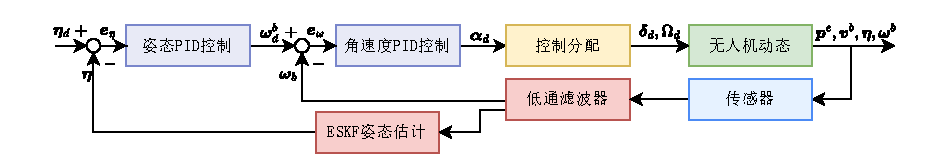
\includegraphics{figure/chapter5/姿态环PID.pdf}
    \caption{姿态PID闭环控制系统框图}
    \label{fig:angle_PID}
\end{figure}

角速度环以机体坐标系下的角速度 \(\boldsymbol{\omega}^b = [p, q, r]^T\) 为被控量。三个通道各自独立使用一个PID控制器，控制器的输出为期望的控制力矩 \(\boldsymbol{M}_d\in\mathbb{R}^3\)。设期望角速度为 \(\boldsymbol{\omega}_d^b\)，则角速度误差为 \(\boldsymbol{e}_{\boldsymbol{\omega}} = \boldsymbol{\omega}_d^b - \boldsymbol{\omega}^b\)。第 \(i\) 个通道的PID控制律可表示为：
\begin{equation}
M_{cv,i} = K_{p,\omega_i} e_{\omega,i} + K_{i,\omega_i} \int e_{\omega,i}\, dt + K_{d,\omega_i} \frac{d e_{\omega,i}}{dt}, \quad i = p,q,r.
\end{equation}

姿态环以欧拉角 \(\boldsymbol{\eta} = [\varphi, \theta, \psi]^T\) 为被控量，其输出作为角速度环的期望值。设期望姿态为 \(\boldsymbol{\eta}_d\)，姿态误差为 \(\boldsymbol{e}_{\boldsymbol{\eta}} = \boldsymbol{\eta}_d - \boldsymbol{\eta}\)。姿态环PID控制器根据姿态误差生成期望角速度 \(\boldsymbol{\omega}_d^b\)：
\begin{equation}
\boldsymbol{\omega}_d^b = K_{p,\eta} \boldsymbol{e}_{\boldsymbol{\eta}} + K_{i,\eta} \int \boldsymbol{e}_{\boldsymbol{\eta}}\, dt + K_{d,\eta} \frac{d \boldsymbol{e}_{\boldsymbol{\eta}}}{dt}.
\end{equation}

\subsection{外环控制器}

外环控制器包括速度环与位置环，用于实现期望的位置与速度跟踪。

\begin{figure}[htbp]
    \centering
    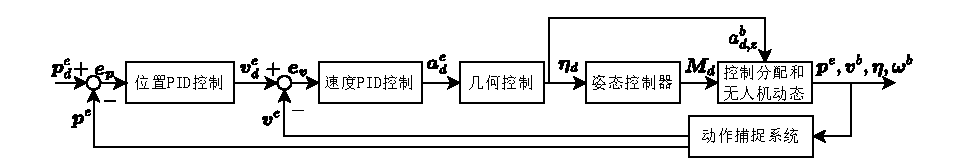
\includegraphics{figure/chapter5/位置环PID.pdf}
    \caption{位置PID闭环控制系统框图}
    \label{fig:pos_PID}
\end{figure}

速度环以地面坐标系下的速度 \(\boldsymbol{v}^e = [v_x^e, v_y^e, v_z^e]^T\) 为被控量，其输出为期望加速度在世界坐标系下的投影 \(\boldsymbol{a}_d^e\)。设期望速度为 \(\boldsymbol{v}_d\)，速度误差为 \(\boldsymbol{e}_{\boldsymbol{v}} = \boldsymbol{v}_d - \boldsymbol{v}\)，则速度环PID控制律为：
\begin{equation}
\boldsymbol{a}_d^e = K_{p,v} \boldsymbol{e}_{\boldsymbol{v}} + K_{i,v} \int \boldsymbol{e}_{\boldsymbol{v}}\, dt + K_{d,v} \frac{d \boldsymbol{e}_{\boldsymbol{v}}}{dt}.
\end{equation}

位置环以地面坐标系下的位置 \(\boldsymbol{p}^e = [p_x^e, p_y^e, p_z^e]^T\) 为被控量，其输出作为速度环的期望值。设期望位置为 \(\boldsymbol{p}_d\)，位置误差为 \(\boldsymbol{e}_{\boldsymbol{p}} = \boldsymbol{p}_d - \boldsymbol{p}\)，则位置环PID控制律为：
\begin{equation}
\boldsymbol{v}_d = K_{p,p} \boldsymbol{e}_{\boldsymbol{p}} + K_{i,p} \int \boldsymbol{e}_{\boldsymbol{p}}\, dt + K_{d,p} \frac{d \boldsymbol{e}_{\boldsymbol{p}}}{dt}.
\end{equation}

值得注意的是，内环的输入为期望姿态 \(\boldsymbol{\eta}_d\)，而外环的输出为期望加速度 \(\boldsymbol{a}_d^e\)。为实现两者的衔接，需采用几何控制算法将期望加速度转换为期望姿态。具体而言，由于涵道无人机是欠驱动系统，平动加速度主要由总推力向量在空间中的指向决定。因此，算法需要将期望加速度 $\boldsymbol{a}_d^e$ 分解为沿机体轴向的期望推力加速度 $a_{d,z}^b$ 以及用于确定机体指向的方向向量。该方向向量结合当前旋转矩阵，进一步解算出无人机达成该加速度所需的期望姿态角 $\boldsymbol{\eta}_d$，从而实现了从外环平动需求到内环转动指令的物理映射。该几何变换保证了外环输出的加速度指令能够被内环姿态控制器有效执行。

所有PID控制器的参数均通过试凑法进行整定，并在实际飞行试验中进行了迭代优化。实验表明，尽管涵道无人机受到地面效应或外部气流的扰动，由于PID的鲁棒性，基于该串级PID控制器的涵道式无人机系统依然能够在悬停点附近稳定飞行，具有良好的鲁棒性和动态响应特性。

% \section{涵道式无人机的PID控制器设计}

% 本文设计的控制器在PID控制器的基础上作优化，本小节介绍串级PID控制器
% 本节的控制器是位置，速度，姿态，角速度的串级PID控制器。
% 简单介绍PID控制器是什么，PID的优势。
% PID分为外环位置速度环和内环姿态角速度环，分别如图\ref{fig:angle_PID}和图\ref{fig:pos_PID}所示。
% 接下来从内到外依次阐述

% \begin{figure}
%     \centering
%     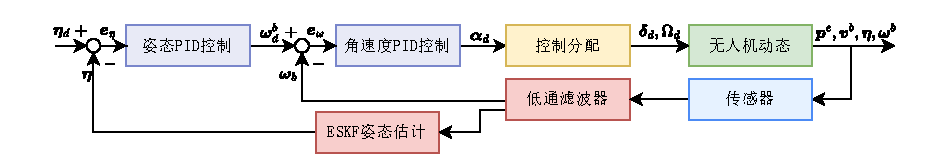
\includegraphics{figure/chapter5/姿态环PID.pdf}
%     \caption{\label{fig:angle_PID}姿态PID闭环控制系统框图}
% \end{figure}
% 该框图构成姿态闭环控制系统。

% \begin{figure}
%     \centering
%     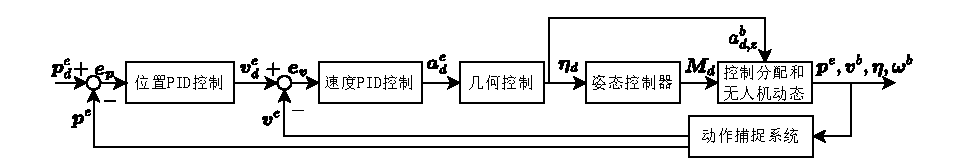
\includegraphics{figure/chapter5/位置环PID.pdf}
%     \caption{\label{fig:pos_PID}位置PID闭环控制系统框图}
% \end{figure}

% \subsection{内环控制器}
% 角速度环以\(\boldsymbol{\omega}^b = [p, q, r]^T\)为被控量。
% 三个被控量各自使用一个PID控制器，以$\boldsymbol{M}_d$为输出量。
% 设期望角速度为 \(\boldsymbol{\omega}_d^b\)，角速度误差为 \(\boldsymbol{e}_\boldsymbol{\omega} = \boldsymbol{\omega}_d^b - \boldsymbol{\omega}^b\)。

% 姿态环以欧拉角 \(\boldsymbol{\eta} = [\varphi, \theta, \psi]^T\) 为被控量。以期望角速度$\boldsymbol{\omega}^b$为输出量。
% 设期望姿态为 \(\boldsymbol{\eta}_d\)，姿态误差为 \(\boldsymbol{e}_\boldsymbol{\eta} = \boldsymbol{\eta}_d - \boldsymbol{\eta}\)。

% \subsection{外环控制器}
% 速度环以\(\boldsymbol{v}^e\)为被控量。
% 三个被控量各自使用一个PID控制器，以$\boldsymbol{a}_{d}^e$为输出量，即期望加速度在世界坐标系下的投影。
% 设期望速度为 \(\boldsymbol{v}_d\)，速度误差为 \(\boldsymbol{e}_\boldsymbol{v} = \boldsymbol{v}_d - \boldsymbol{v}\)。

% 值得注意的是，内环的输入为期望姿态$\boldsymbol{\eta}_d$，而外环的输出是期望加速度\(\boldsymbol{a}_d^e\)。因此，需要经过几何控制算法，将该加速度的分解为方向向量和沿机体轴的加速度\(a_{d,z}^b\)，方向向量在根据当前旋转矩阵和转换为无人机的期望姿态$\boldsymbol{\eta}_d$。

% 所有PID控制器的参数均通过试凑法进行整定，并在仿真与实际飞行试验中进行了迭代优化。实验表明，尽管涵道无人机受到地面效应或外部气流的扰动，由于PID的鲁棒性，该基于该PID，无人机系统依然能够在悬停点稳定。
\section{地面效应控制补偿}
\label{sec:ge_compensate}

本小节旨在将第四章离线辨识得到的地面效应模型应用于飞行控制系统中，实现对控制分配器的动态补偿。根据第四章建立的半经验模型，涵道式无人机在近地面飞行时，其推力系数 \(K_T\) 与控制舵面偏转力系数 \(K_{cv}\) 均随无量纲离地高度 \(h/R\) 发生显著变化，分别演变为与高度相关的函数 \(K_{TGE}(h/R)\) 和 \(K_{cvGE}(h/R)\)。若在控制器中仍沿用无地效状态下的恒定系数，将导致模型失配，使得实际产生的推力和力矩偏离期望值，进而影响控制精度甚至引发系统振荡。

因此，抗地面效应控制补偿的核心在于：在控制分配环节，利用机载激光测距模块实时获取的离地高度信息，动态更新控制效率矩阵中的气动系数。具体而言，用实时计算得到的 \(K_{TGE}\) 和 \(K_{cvGE}\) 替换原控制效率矩阵 \(\boldsymbol{B}\) 中的 \(K_T\) 和 \(K_{cv}\)，从而构建考虑地面效应影响的修正控制效率矩阵 \(\boldsymbol{B}_{GE}\)：
\begin{equation}
    \boldsymbol{B}_{GE} = 
    \begin{bmatrix}
        K_{TGE} & 0 & 0 & 0 & 0 \\
        0 & -K_{cvGE} l_1 & 0 & K_{cvGE} l_1 & 0 \\
        0 & 0 & -K_{cvGE} l_1 & 0 & K_{cvGE} l_1 \\
        0 & K_{cvGE} l_2 & K_{cvGE} l_2 & K_{cvGE} l_2 & K_{cvGE} l_2
    \end{bmatrix},
    \label{eq:B_GE}
\end{equation}
其中，\(K_{TGE}\) 与 \(K_{cvGE}\) 采用第四章辨识得到的指数模型进行估计，具体表达式为：
\begin{equation}
    K_{TGE} = K_{T}\left(1 + 0.378 \cdot e^{-1.105 \cdot (h/R)}\right),
    \label{eq:KTGE}
\end{equation}
\begin{equation}
    K_{cvGE} = K_{cv}\left(1 - 0.950 \cdot e^{-1.174 \cdot (h/R)}\right).
    \label{eq:K_cvGE}
\end{equation}

上述两式中，\(K_T\) 和 \(K_{cv}\) 分别为无地效状态下的基准推力系数与舵面偏转力系数，其数值由表2-2给出。在飞行过程中，将实时测得的离地高度 \(h\) 代入式\eqref{eq:KTGE}与式\eqref{eq:K_cvGE}，即可在线计算当前高度下的实际气动系数，进而通过式\eqref{eq:B_GE}更新控制效率矩阵。在控制分配环节，将 \(\boldsymbol{B}_{GE}\) 代入伪逆分配律式\eqref{eq:B_matrix}，即可实现期望推力与力矩向执行器指令的准确映射。实验结果表明，该方法能够补偿绝大部分由地面效应引起的推力与舵效变化，有效抑制了近地面飞行时的垂向振荡与姿态漂移。

值得注意的是，推力补偿模型的实现还需考虑执行器层面的映射关系。由式\eqref{eq:KTGE}可知，在给定期望推力 \(T_{d}\) 的情况下，期望螺旋桨转速 \(\Omega_d\) 可通过下式解算：
\begin{equation}
    \Omega_d = \sqrt{\frac{T_{d}}{K_{TGE}}}.
    \label{eq:omega_from_thrust}
\end{equation}

然而，飞控系统实际输出的是电机的油门百分比指令 \(t_{motor}\)，且螺旋桨转速与油门百分比之间的关系受电池电压影响显著。为建立准确的转速-油门映射，本文在恒定电压 \(V_{ref}=13.00\,\mathrm{V}\) 的条件下开展了静态台架实验，通过采集不同油门百分比下的稳态转速数据，拟合得到如下线性关系：
\begin{equation}
\Omega = 1115.01 \cdot t_{motor} + 158.8,
\end{equation}
其中 \(\Omega_d\) 的单位为 \(\mathrm{rad/s}\)，\(V_{bat}\) 的单位为 \(\mathrm{V}\)，\(t_{motor}\) 为取值在 \([0, 1]\) 范围内的油门输出百分比。实际飞行中电池电压 \(V_{bat}\) 会随放电而波动，导致相同油门百分比下的转速发生变化。根据无刷直流电机的调速特性，引入电压补偿系数 \(13.00 / V_{bat}\) 对期望转速进行修正。综合上述关系，由期望转速 \(\Omega_d\) 反解油门百分比的表达式为：
\begin{equation}
    t_{motor} = \frac{\Omega_d - 158.8}{1115.01} \cdot \frac{13.00}{V_{bat}},
    \label{eq:throttle_mapping}
\end{equation}
其中\(V_{bat}\) 的单位为 \(\mathrm{V}\)。

为验证该补偿策略的有效性，在静态台架上开展了转速跟踪实验。实验中，飞控系统根据预设的目标转速序列，通过式\eqref{eq:throttle_mapping}实时计算油门指令并驱动电机运行，同时通过无刷电机测速模块记录实际转速。图\ref{fig:speed_tracking}展示了在电池电压存在轻微波动情况下，目标转速与实际转速的跟踪曲线。同时记录电池电压的实时波动情况如图\ref{fig:battery_voltage}所示。
\begin{figure}[htbp]
    \centering
    \begin{minipage}[b]{0.45\textwidth}
        \centering
        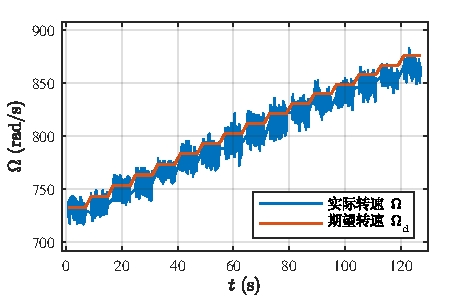
\includegraphics{matlab/ground_effect/pdf/anti_ge_thrust/Plot_Speed_Tracking_speed_track.pdf}
        \caption{实际转速与期望转速的跟随曲线}
        \label{fig:speed_tracking}
    \end{minipage}
    \hfill  % 产生弹性水平间距
    \begin{minipage}[b]{0.45\textwidth}
        \centering
        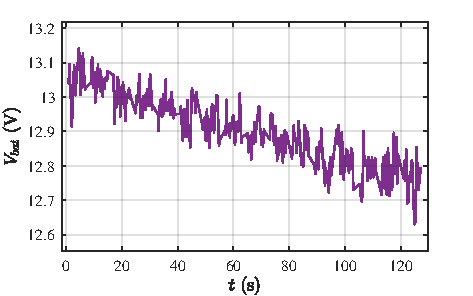
\includegraphics{matlab/ground_effect/pdf/anti_ge_thrust/Plot_Battery_Voltage_speed_track.pdf}
        \caption{实验过程电压波动曲线}
        \label{fig:battery_voltage}
    \end{minipage}
\end{figure}

从图中可以看出，实际转速能够快速跟随目标转速的变化，稳态跟踪误差小，动态响应迅速。即使在电压波动条件下，由于电压补偿系数的引入，转速跟踪依然保持了较高精度$(3\,\%)$以内。实验验证了式\eqref{eq:throttle_mapping}所描述的转速-油门映射关系在实际系统中的工程有效性。

% \section{地面效应控制补偿}

% 简短介绍本小节做的内容。依照第四章建立的模型，无人机的升力系数$K_{TGE}$和偏转力系数$K_{cvGE}$是离地高度比$h/R$的函数。因此抗地面效应控制补偿的核心在于，在控制分配环节，使用实时变化的$K_{TGE}$和$K_{cvGE}$替换$\boldsymbol{B}$矩阵中的$K_T$和$K_{cv}$，那么考虑地效影响下更新后的控制效率矩阵$\boldsymbol{B}_{GE}$为：
% \begin{equation}
%     \boldsymbol{B} = 
%     \begin{bmatrix}
%         K_{TGE} & 0 & 0 & 0 & 0 \\
%         0 & -K_{cvGE} l_1 & 0 & K_{cvGE} l_1 & 0 \\
%         0 & 0 & -K_{cvGE} l_1 & 0 & K_{cvGE} l_1 \\
%         0 & K_{cvGE} l_2 & K_{cvGE} l_2 & K_{cvGE} l_2 & K_{cvGE} l_2
%     \end{bmatrix}.
% \end{equation}
% 其中，$K_{TGE}$，$K_{cvGE}$使用第四章拟合的模型来估计，即满足：
% \begin{equation}
%     K_{TGE} = K_{T}\left(1 + 0.378 \cdot e^{-1.105 \cdot (h/R)}\right),
% \end{equation}
% \begin{equation}
%     K_{cvGE} = K_{cv}\left(1 - 0.950 \cdot e^{-1.174 \cdot (h/R)}\right).
% \end{equation}

% 通过该方法能够补偿绝大部分地面效应带来的扰动。

% 值得注意的是，针对推力的补偿模型中，根据：
% $T_{GE} = K_{TGE} * \Omega ^2,$
% 在给定期望推力的前提下，能够通过该式计算出期望螺旋桨转速$\Omega_d$。
% 由于无人机飞行过程中存在电池电压不恒定的情况，因此需要找出螺旋桨期望转速转速$\Omega_d$和电池电压$V_{bat}$以及电机油门输出百分比$t_{motor}$之间的关系。本文经过拟合，直接给出其关系为：
% \begin{equation}
%     t_{motor} = (\Omega_d - 158.8) / 1115.01 * 13.00 / V_{bat}
% \end{equation}
% 其中，$\Omega_d$的单位是$\mathrm{rad/s}$，$V_{bat}$的单位是$\mathrm{V}$，$t_{motor}$是范围为$[0,\, 1]$的油门输出百分比。经实验验证该算法能够对螺旋桨转速实现有效的开环控制。
\subsection{推力补偿效果实验}
\label{sec:thrust_experiment}
基于第\ref{sec:ge_compensate}节所介绍的地面效应补偿方法，本小节在静态台架上开展推力补偿效果验证实验，以检验该补偿算法在期望推力生成方面的有效性。

实验平台与第四章地面效应辨识实验保持一致，主要由以下部分组成：可编程数字直流电源，六维力/力矩传感器，实验样机，气流约束板。

\subsubsection{实验工况与步骤}

实验分为两组进行：第一组为实验组，部署第\ref{sec:ge_compensate}节所设计的推力补偿算法；第二组为对照组，在相同实验环境下不进行推力补偿，直接采用无地效状态下的恒定推力系数进行控制分配。通过对比两组实验在给定期望推力的前提下实际产生的推力大小，评估补偿算法的有效性。

具体实验步骤如下：

\textbf{1. 传感器校准}：在实验开始前，对六维力/力矩传感器进行静态校准。在无人机未通电、螺旋桨静止的状态下，以 \(200\,\mathrm{Hz}\) 的采样频率连续采集传感器输出 \(5\,\mathrm{s}\)，并将该时间段内各通道测量值的平均值作为该次实验的静态零点偏置。该偏置值将在后续数据处理中予以扣除，以消除传感器零点漂移和无人机自重对测量结果的影响。
    
\textbf{2. 高度工况设定}：根据涵道风扇地面效应的作用范围，选取三个具有代表性的离地高度进行测试，分别为 \(h = 50\,\mathrm{mm}\)、\(100\,\mathrm{mm}\) 和 \(200\,\mathrm{mm}\)，对应的无量纲高度比分别为 \(h/R = 0.56\)、\(1.12\) 和 \(2.25\)。其中 \(h/R = 0.56\) 处于强地面效应区，\(h/R = 1.12\) 处于地效过渡区，\(h/R = 2.25\) 处于弱地效区。通过调节龙门架上的竖直导轨，将气流约束板依次固定至各高度位置。
    
\textbf{3. 期望推力序列设定}：在每个固定的离地高度下，依次给控制分配模块设定一系列期望推力值 \(T_d\)。期望推力的设定范围覆盖无人机悬停工况及小幅度加减速工况，以悬停推力 \(T_{\mathrm{hover}} = 4.48\,\mathrm{N}\)为中心，在 \(3.5\,\mathrm{N}\) 至 \(5.0\,\mathrm{N}\) 范围内，以\(0.1\,\mathrm{N}\)为步长均匀选取多个测试点。控制分配模块根据当前高度下的地面效应模型，通过式\eqref{eq:omega_from_thrust}解算期望螺旋桨转速 \(\Omega_d\)。
    
\textbf{4. 执行器指令映射}：将解算得到的期望转速 \(\Omega_d\) 代入转速-油门映射关系式\eqref{eq:throttle_mapping}，结合实时采集的电池电压 \(V_{bat}\)，计算出对应的电机油门百分比指令 \(t_{motor}\)，并通过飞控系统输出至电机电调。
    
\textbf{5. 数据采集}：在每个期望推力指令发出后，等待 \(2\,\mathrm{s}\) 以使电机转速建立稳态，随后以 \(200\,\mathrm{Hz}\) 的采样频率连续记录以下数据：力传感器实测推力值 \(T\)、期望推力值 \(T_d\)、螺旋桨期望转速 \(\Omega_d\)以及螺旋桨实际转速 \(\Omega\) 。每个工况点的数据记录时长为 \(8\,\mathrm{s}\)，以保证后续统计平均处理的有效性。
    
\textbf{6. 重复性实验}：为消除随机误差对实验结果的影响，每个高度下的每个期望推力点均重复实验至少三次，取三次测量的平均值作为该工况下的最终推力输出值。


实验结束后，将采集的数据导出至计算机进行离线处理与分析，通过对比实验组与对照组在不同高度下的推力输出误差，定量评估推力补偿算法的有效性。

% \subsection{验证推力补偿效果实验}
% 基于\ref{sec:ge_compensate}小节介绍的补偿方法，本小节在静态台架上，通过实验验证该方式的补偿效果。
% 实验与第四章使用同样的测试平台，平台主要由学生电源，力矩传感器，实验样机以及约束板构成。

% 实验分为两组进行，一组部署推力补偿算法，一组则作为对照组，在相同环境下不进行推力补偿，比较两组实验在给定期望推力的前提下，实际产生的推力大小。
% 实验步骤如下：
% 1、力传感器静态校准，采集静态输出5s，取均值，作为该传感器的静态偏置。
% 2、将气流约束板依次放在50，100，200mm高度，分别对应h/R = 0.56， 1.12， 2.25，用于验证能否输出期望力矩。涵盖从强地面效应区到弱地效区的范围
% 3、在每个独立的高度下，从弱到强，依次给控制分配模块依次设定期望推力$T_d$，根据样机重量，悬停推力为$4.48$N，控制分配模块解算当前需要的螺旋桨转速$\Omega_d$。
% 4、再通过螺旋桨的开环控制，解算出需要的电机油门。
% 5、实验过程全程将力传感器推力值$T$，期望推力值$T_d$，螺旋桨期望转速$\Omega_d$、螺旋桨实际转速$\Omega$，按照200Hz的频率采集。
% 6、根据上述步骤每个高度下，重复实验至少三次，以排除实验误差

\subsubsection{实验数据}

按照上述实验步骤完成数据采集与预处理后，本小节对推力补偿效果进行定量分析与可视化展示。实验数据覆盖三个典型无量纲高度 \(h/R = 0.56\)、\(1.12\) 和 \(2.25\)，在每个高度下，通过对比推力补偿算法部署前后的实际推力输出与螺旋桨转速跟踪情况，验证补偿方法的有效性。

% \subsubsection{实验数据}
% 按照上述实验步骤完成数据采集与预处理后，本小节对推力补偿效果进行定量分析与可视化展示。

% 为了展示推力补偿的效果，可将各个高度下期望力矩$T_d$，和经过补偿后采集到的推力大小$T$以及未经过补偿时采集到的推力大小$T^{\prime}$绘制在同一图上，如图\ref{fig:50mmThrust_Tracking,fig:100mmThrust_Tracking,fig:200mmThrust_Tracking}所示

% 此外为了直观展示出$K_{TGE}$变化带来的效果，也为了排除螺旋桨转速$\Omega$未达到期望转速$\Omega_d$的干扰，本小节将各个高度下，在未使用推力补偿时解算出的螺旋桨期望转速$\Omega_d^{prime}$及其实际转速$\Omega^{prime}$，和使用推力补偿时解算出的螺旋桨期望转速$\Omega_d$及其实际转速$\Omega$绘制同一图上，如图\ref{fig:50mmSpeed_Tracking, fig:100mmSpeed_Tracking, fig:200mmSpeed_Tracking}所示。

\begin{figure}[htbp]
    \centering
    \begin{minipage}[b]{0.45\textwidth}
        \centering
        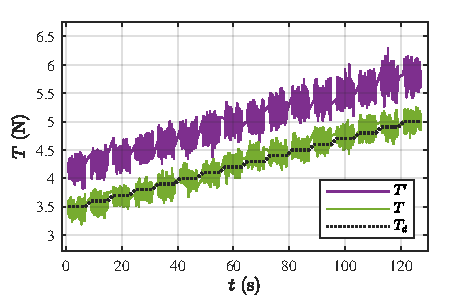
\includegraphics{matlab/ground_effect/pdf/anti_ge_thrust/Plot_Thrust_Tracking_50mm.pdf}
        \caption{$h/R = 0.56$，期望推力与实际推力}
        \label{fig:50mmThrust_Tracking}
    \end{minipage}
    \hfill  % 产生弹性水平间距
    \begin{minipage}[b]{0.45\textwidth}
        \centering
        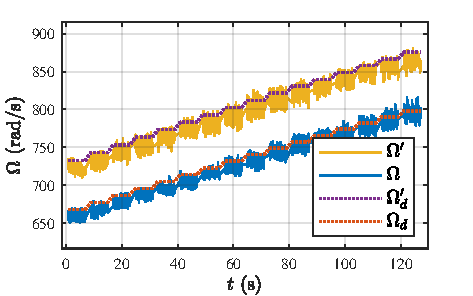
\includegraphics{matlab/ground_effect/pdf/anti_ge_thrust/Plot_Speed_Tracking_50mm.pdf}
        \caption{$h/R = 0.56$，期望转速与实际转速}
        \label{fig:50mmSpeed_Tracking}
    \end{minipage}
\end{figure}


\begin{figure}[htbp]
    \centering
    \begin{minipage}[b]{0.45\textwidth}
        \centering
        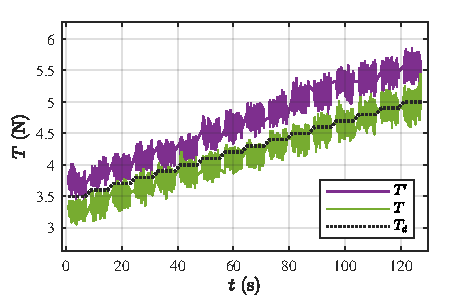
\includegraphics{matlab/ground_effect/pdf/anti_ge_thrust/Plot_Thrust_Tracking_100mm.pdf}
        \caption{$h/R=1.12$，期望推力与实际推力}
        \label{fig:100mmThrust_Tracking}
    \end{minipage}
    \hfill  % 产生弹性水平间距
    \begin{minipage}[b]{0.45\textwidth}
        \centering
        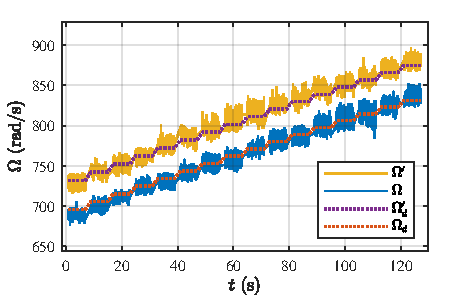
\includegraphics{matlab/ground_effect/pdf/anti_ge_thrust/Plot_Speed_Tracking_100mm.pdf}
        \caption{$h/R=1.12$，期望转速与实际转速}
        \label{fig:100mm_Speed_Tracking}
    \end{minipage}
\end{figure}


\begin{figure}[htbp]
    \centering
    \begin{minipage}[b]{0.45\textwidth}
        \centering
        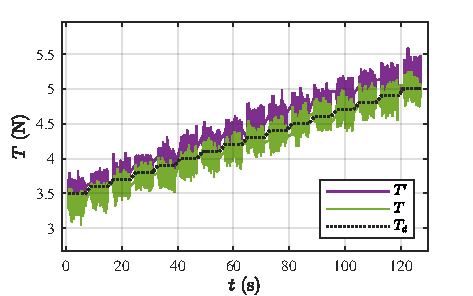
\includegraphics{matlab/ground_effect/pdf/anti_ge_thrust/Plot_Thrust_Tracking_200mm.pdf}
        \caption{$h/R=2.25$，期望推力与实际推力}
        \label{fig:200mmThrust_Tracking}
    \end{minipage}
    \hfill  % 产生弹性水平间距
    \begin{minipage}[b]{0.45\textwidth}
        \centering
        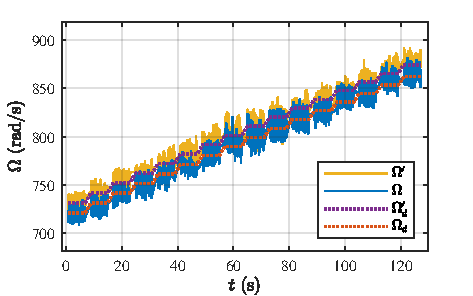
\includegraphics{matlab/ground_effect/pdf/anti_ge_thrust/Plot_Speed_Tracking_200mm.pdf}
        \caption{$h/R=2.25$，期望转速与实际转速}
        \label{fig:200mmSpeed_Tracking}
    \end{minipage}
\end{figure}

为直观展示推力补偿效果，将各高度下期望推力 \(T_d\)、经补偿后实测推力 \(T\) 以及未补偿时实测推力 \(T'\) 绘制于同一图中，结果如图\ref{fig:50mmThrust_Tracking}、图\ref{fig:100mmThrust_Tracking}和图\ref{fig:200mmThrust_Tracking}所示。从图中可以观察到，在未施加推力补偿的情况下，实测推力 \(T'\) 与期望推力 \(T_d\) 之间存在显著偏差：在强地效区（\(h/R = 0.56\)），实际输出推力较期望值偏大约 \(20\%\)～\(25\%\)；在地效过渡区（\(h/R = 1.12\)），偏差缩小至 \(10\%\) 左右；在弱地效区（\(h/R = 2.25\)），偏差进一步减小至 \(5\%\) 以内。这一现象与第四章地面效应辨识结果一致：近地面时涵道风扇实际推力高于无地效基准值，且偏差随高度降低而增大。相比之下，采用推力补偿算法后，实测推力 \(T\) 与期望推力 \(T_d\) 在各高度下均表现出良好的一致性，稳态误差能够稳定控制在 \(5\%\) 以内，验证了补偿模型的有效性。

为进一步排除螺旋桨转速跟踪误差对推力输出结果的干扰，直观展示 \(K_{TGE}\) 动态补偿的作用机理，本小节将各高度下两组实验的螺旋桨期望转速与实际转速进行对比分析。具体而言，记录未使用推力补偿时解算的期望转速 \(\Omega_d'\) 及其实际转速 \(\Omega'\)，以及使用推力补偿时解算的期望转速 \(\Omega_d\) 及其实际转速 \(\Omega\)，绘制结果如图\ref{fig:50mmSpeed_Tracking}、图\ref{fig:100mm_Speed_Tracking}和图\ref{fig:200mmSpeed_Tracking}所示。
\subsection{控制舵面偏转力补偿效果实验}

基于第\ref{sec:ge_compensate}节所介绍的地面效应补偿方法，本小节在静态台架上开展舵面偏转力补偿效果验证实验，以检验补偿算法在给定期望力矩条件下的实际输出精度。实验平台与推力补偿实验相同，主要包括可编程数字直流电源、六维力/力矩传感器、实验样机及气流约束板。

\subsubsection{实验工况与步骤}

实验分为两组：实验组部署第\ref{sec:ge_compensate}节设计的舵面偏转力补偿算法，在控制分配环节采用随高度变化的舵面偏转力系数 \(K_{cvGE}\)；对照组不进行补偿，始终采用无地效状态下的恒定系数 \(K_{cv}\)。通过对比两组实验在给定期望扭矩下实际输出的 \(Z\) 轴扭矩 \(M_z\)，评估补偿算法的有效性。

具体实验步骤如下：

\textbf{1. 传感器校准}：实验开始前，在无人机未通电、螺旋桨静止的状态下，以 \(200\,\mathrm{Hz}\) 采样频率连续采集传感器输出 \(5\,\mathrm{s}\)，取各通道平均值作为静态零点偏置，用于后续数据修正。
    
\textbf{2. 高度工况设定}：选取三个典型无量纲高度 \(h/R = 0.56\)、\(1.12\) 和 \(2.25\)，分别对应强地效区、地效过渡区与弱地效区。通过调节竖直导轨将气流约束板依次固定至各高度位置。
    
\textbf{3. 期望扭矩序列设定}：在每个固定高度下，向控制分配模块依次施加一系列期望扭矩 \(M_{z,d}\)，取值范围为 \([-0.04, 0.04]\,\mathrm{N\cdot m}\)，以 \(0.008\,\mathrm{N\cdot m}\) 为步长均匀选取多个测试点。控制分配模块根据当前高度下的地面效应模型式\eqref{eq:KcvGE}，通过式\eqref{eq:B_GE}解算期望舵面偏转角 \(\boldsymbol{\delta}_d\)。由于仅存在 \(Z\) 轴期望力矩，根据式\eqref{eq:B_matrix}可知，四个舵面偏转角应保持一致，即 \(\boldsymbol{\delta}_d = [\delta_d,\delta_d,\delta_d,\delta_d]^T\)。
    
\textbf{4. 数据采集}：在每个期望扭矩指令发出后，等待 \(2\,\mathrm{s}\) 以使气流建立稳态，随后以 \(200\,\mathrm{Hz}\) 采样频率连续记录实测 \(Z\) 轴扭矩 \(M_z\) 与期望扭矩 \(M_{z,d}\)，每个工况点记录时长 \(7\,\mathrm{s}\)。
    
\textbf{5. 重复性实验}：为消除随机误差，每个高度下的每个期望扭矩点均重复实验至少三次，取三次测量的平均值作为该工况下的最终 \(M_z\) 输出值。

实验结束后，将采集数据导出至计算机进行离线处理与分析，通过对比实验组与对照组在不同高度下的 \(M_z\) 输出误差，定量评估舵面偏转力补偿算法的有效性。

\subsubsection{实验数据}

按照上述实验步骤完成数据采集与预处理后，本小节对舵面偏转力补偿效果进行定量分析与可视化展示。实验数据覆盖三个典型无量纲高度 \(h/R = 0.56\)、\(1.12\) 和 \(2.25\)，在每个高度下，通过对比补偿算法部署前后的实际 \(Z\) 轴扭矩输出跟踪情况，验证补偿方法的有效性。

\begin{figure}[htbp]
    \centering
    \begin{minipage}[b]{0.45\textwidth}
        \centering
        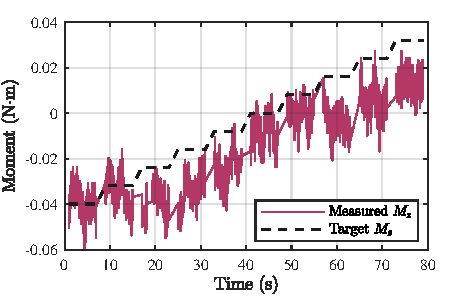
\includegraphics{matlab/ground_effect/pdf/anti_ge_moment/Moment_Tracking_50mm.pdf}
        \caption{$h/R = 0.56$，期望扭矩与实际扭矩}
        \label{fig:moemnt_tracking_50mm}
    \end{minipage}
    \hfill
    \begin{minipage}[b]{0.45\textwidth}
        \centering
        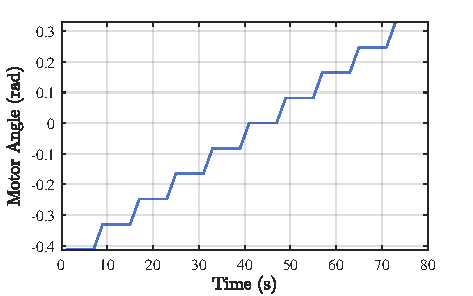
\includegraphics{matlab/ground_effect/pdf/anti_ge_moment/Motor_Angle_50mm.pdf}
        \caption{$h/R = 0.56$，期望舵面偏转角}
        \label{fig:motor_angle_50mm}
    \end{minipage}
\end{figure}

\begin{figure}[htbp]
    \centering
    \begin{minipage}[b]{0.45\textwidth}
        \centering
        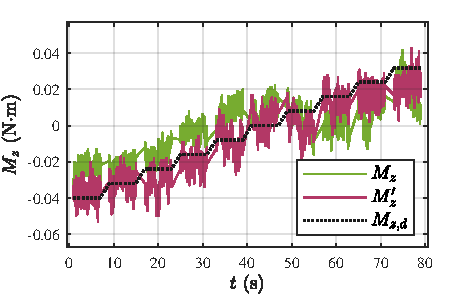
\includegraphics{matlab/ground_effect/pdf/anti_ge_moment/Moment_Tracking_100mm.pdf}
        \caption{$h/R=1.12$，期望扭矩与实际扭矩}
        \label{fig:moemnt_tracking_100mm}
    \end{minipage}
    \hfill
    \begin{minipage}[b]{0.45\textwidth}
        \centering
        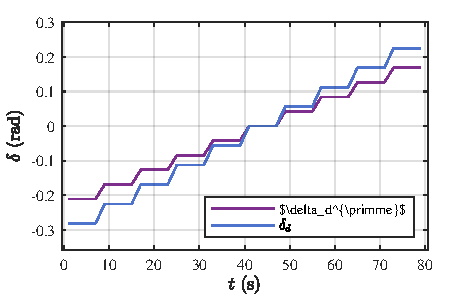
\includegraphics{matlab/ground_effect/pdf/anti_ge_moment/Motor_Angle_100mm.pdf}
        \caption{$h/R=1.12$，期望舵面偏转角}
        \label{fig:motor_angle_100mm}
    \end{minipage}
\end{figure}

\begin{figure}[htbp]
    \centering
    \begin{minipage}[b]{0.45\textwidth}
        \centering
        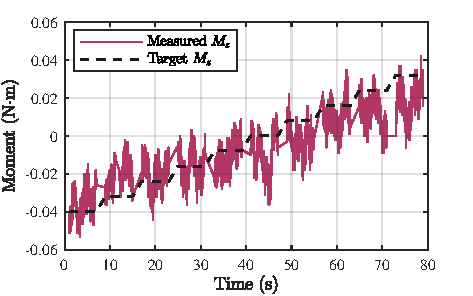
\includegraphics{matlab/ground_effect/pdf/anti_ge_moment/Moment_Tracking_200mm.pdf}
        \caption{$h/R=2.25$，期望扭矩与实际扭矩}
        \label{fig:moemnt_tracking_200mm}
    \end{minipage}
    \hfill
    \begin{minipage}[b]{0.45\textwidth}
        \centering
        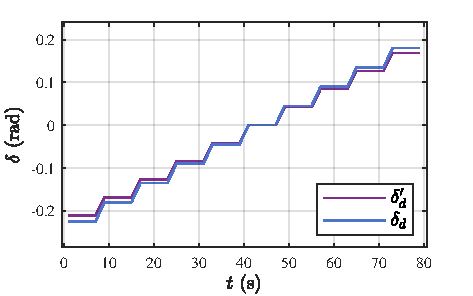
\includegraphics{matlab/ground_effect/pdf/anti_ge_moment/Motor_Angle_200mm.pdf}
        \caption{$h/R=2.25$，期望舵面偏转角}
        \label{fig:motor_angle_200mm}
    \end{minipage}
\end{figure}

为直观展示舵面偏转力补偿效果，将各高度下期望扭矩 \(M_{z,d}\)、补偿后实测扭矩 \(M_z\) 以及未补偿时实测扭矩 \(M_z^{\prime}\) 绘制于同一图中，结果如图\ref{fig:moemnt_tracking_50mm}、\ref{fig:moemnt_tracking_100mm}和\ref{fig:moemnt_tracking_200mm}所示。从图中可以观察到，未施加补偿时，实测扭矩 \(M_z^{\prime}\) 与期望扭矩 \(M_{z,d}\) 存在显著偏差：在强地效区（\(h/R = 0.56\)），实际输出扭矩较期望值偏大约 \(20\%\)～\(25\%\)；在地效过渡区（\(h/R = 1.12\)），偏差缩小至 \(10\%\) 左右；在弱地效区（\(h/R = 2.25\)），偏差进一步减小至 \(5\%\) 以内。这一现象与第四章地面效应辨识结果一致：近地面时舵面偏转力高于无地效基准值，且偏差随高度降低而增大。采用补偿算法后，实测扭矩 \(M_z\) 与期望扭矩 \(M_{z,d}\) 在各高度下均表现出良好的一致性，稳态误差稳定控制在 \(10\%\) 以内，验证了补偿模型的有效性。

为直观展示 \(K_{cvGE}\) 动态补偿的作用机理，本小节将各高度下两组实验的控制舵面期望偏转角进行对比分析。记录未补偿时解算的期望偏转角 \(\delta_d^{\prime}\) 与补偿时解算的期望偏转角 \(\delta_d\)，绘制结果如图\ref{fig:motor_angle_50mm}、\ref{fig:motor_angle_100mm}和\ref{fig:motor_angle_200mm}所示。从图中可以看出，在相同期望扭矩指令下，补偿组解算的期望偏转角 \(\delta_d\) 显著小于未补偿组 \(\delta_d^{\prime}\)。以 \(h/R = 0.56\)、期望扭矩 \(0.03\,\mathrm{N\cdot m}\) 为例，补偿组期望偏转角约为 \(10^\circ\)，而未补偿组约为 \(13^\circ\)，两者相差约 \(3^\circ\)。这正是补偿算法通过动态调整舵面偏角来抵消地效引起的舵面效率增益的具体体现。

\section{涵道式无人机地面效应抗扰控制}
为验证本文所设计的地面效应补偿算法在实际飞行环境中的有效性与鲁棒性，本小节以涵道式无人机实验样机为对象，开展近地面抗扰控制实飞实验。实验在室内动作捕捉系统的有效测量空间内进行，通过对比是否部署地面效应补偿算法时无人机在近地面端的高度位置阶跃响应与偏航角阶跃响应，定量评估推力补偿与舵面偏转力补偿对控制性能的改善效果。

部署上述抗扰算法后，无人机飞行控制系统的局部框图如图\ref{fig:anti_ge_system}所示。几何控制模块根据期望加速度与当前姿态解算期望推力与期望力矩，内环姿态控制器输出期望角加速度。上述期望量共同输入至控制分配模块。控制分配模块首先根据无人机质量 \(m\) 与转动惯量矩阵 \(\boldsymbol{J}\)，将期望加速度与角加速度转换为期望推力 \(T_d\) 与期望控制力矩 \(\boldsymbol{M}_d\)；同时，通过机载激光测距模块实时获取当前离地高度 \(h\)，据此动态更新地面效应下的推力系数 \(K_{TGE}\) 与舵面偏转力系数 \(K_{cvGE}\)，进而构建修正控制效率矩阵 \(\boldsymbol{B}_{GE}\)。最后，采用伪逆法解算执行器期望输出（螺旋桨转速 \(\Omega_d\) 与舵面偏转角 \(\boldsymbol{\delta}_d\)），实现期望控制效应的准确分配。
% 本小节将使用本文研究的涵道式无人机执行实际飞行试验。

% 部署上述抗扰算法后，进行无人机实飞测试。

% 部署抗扰动控制后的实际飞行测试的局部系统框图如下图\ref{fig:anti_ge_system}所示。

% 几何控制输出的期望加速度和内环输出的期望角加速度给到控制分配模块。控制分配模块首先根据无人机的质量$m$和无人机的转动惯量矩阵$\boldsymbol{J}$，将其转换为期望的推力$T_d$以及期望控制力矩$M_d$。并且获取当前离地高度$h$。更新当前系数$K_{TGE}$和$K_{cvGE}$，获取控制效应矩阵$B_{GE}$。从而通过伪逆法计算出执行器的期望输出。

\begin{figure}[htbp]
    \centering
    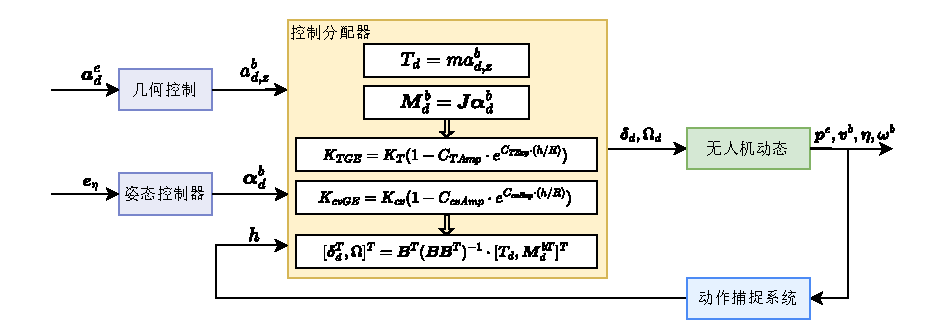
\includegraphics{figure/chapter5/地面效应抗扰控制.pdf}
    \caption{抗扰控制局部系统框图}
    \label{fig:anti_ge_system}
\end{figure}

无人机实际飞行试验过程如图\ref{fig:anti_ge_flight}所示，涵盖了近地面悬停、高度阶跃响应等典型工况。

\begin{figure}[htbp]
    \centering
    \begin{minipage}[b]{0.45\textwidth}
        \centering
        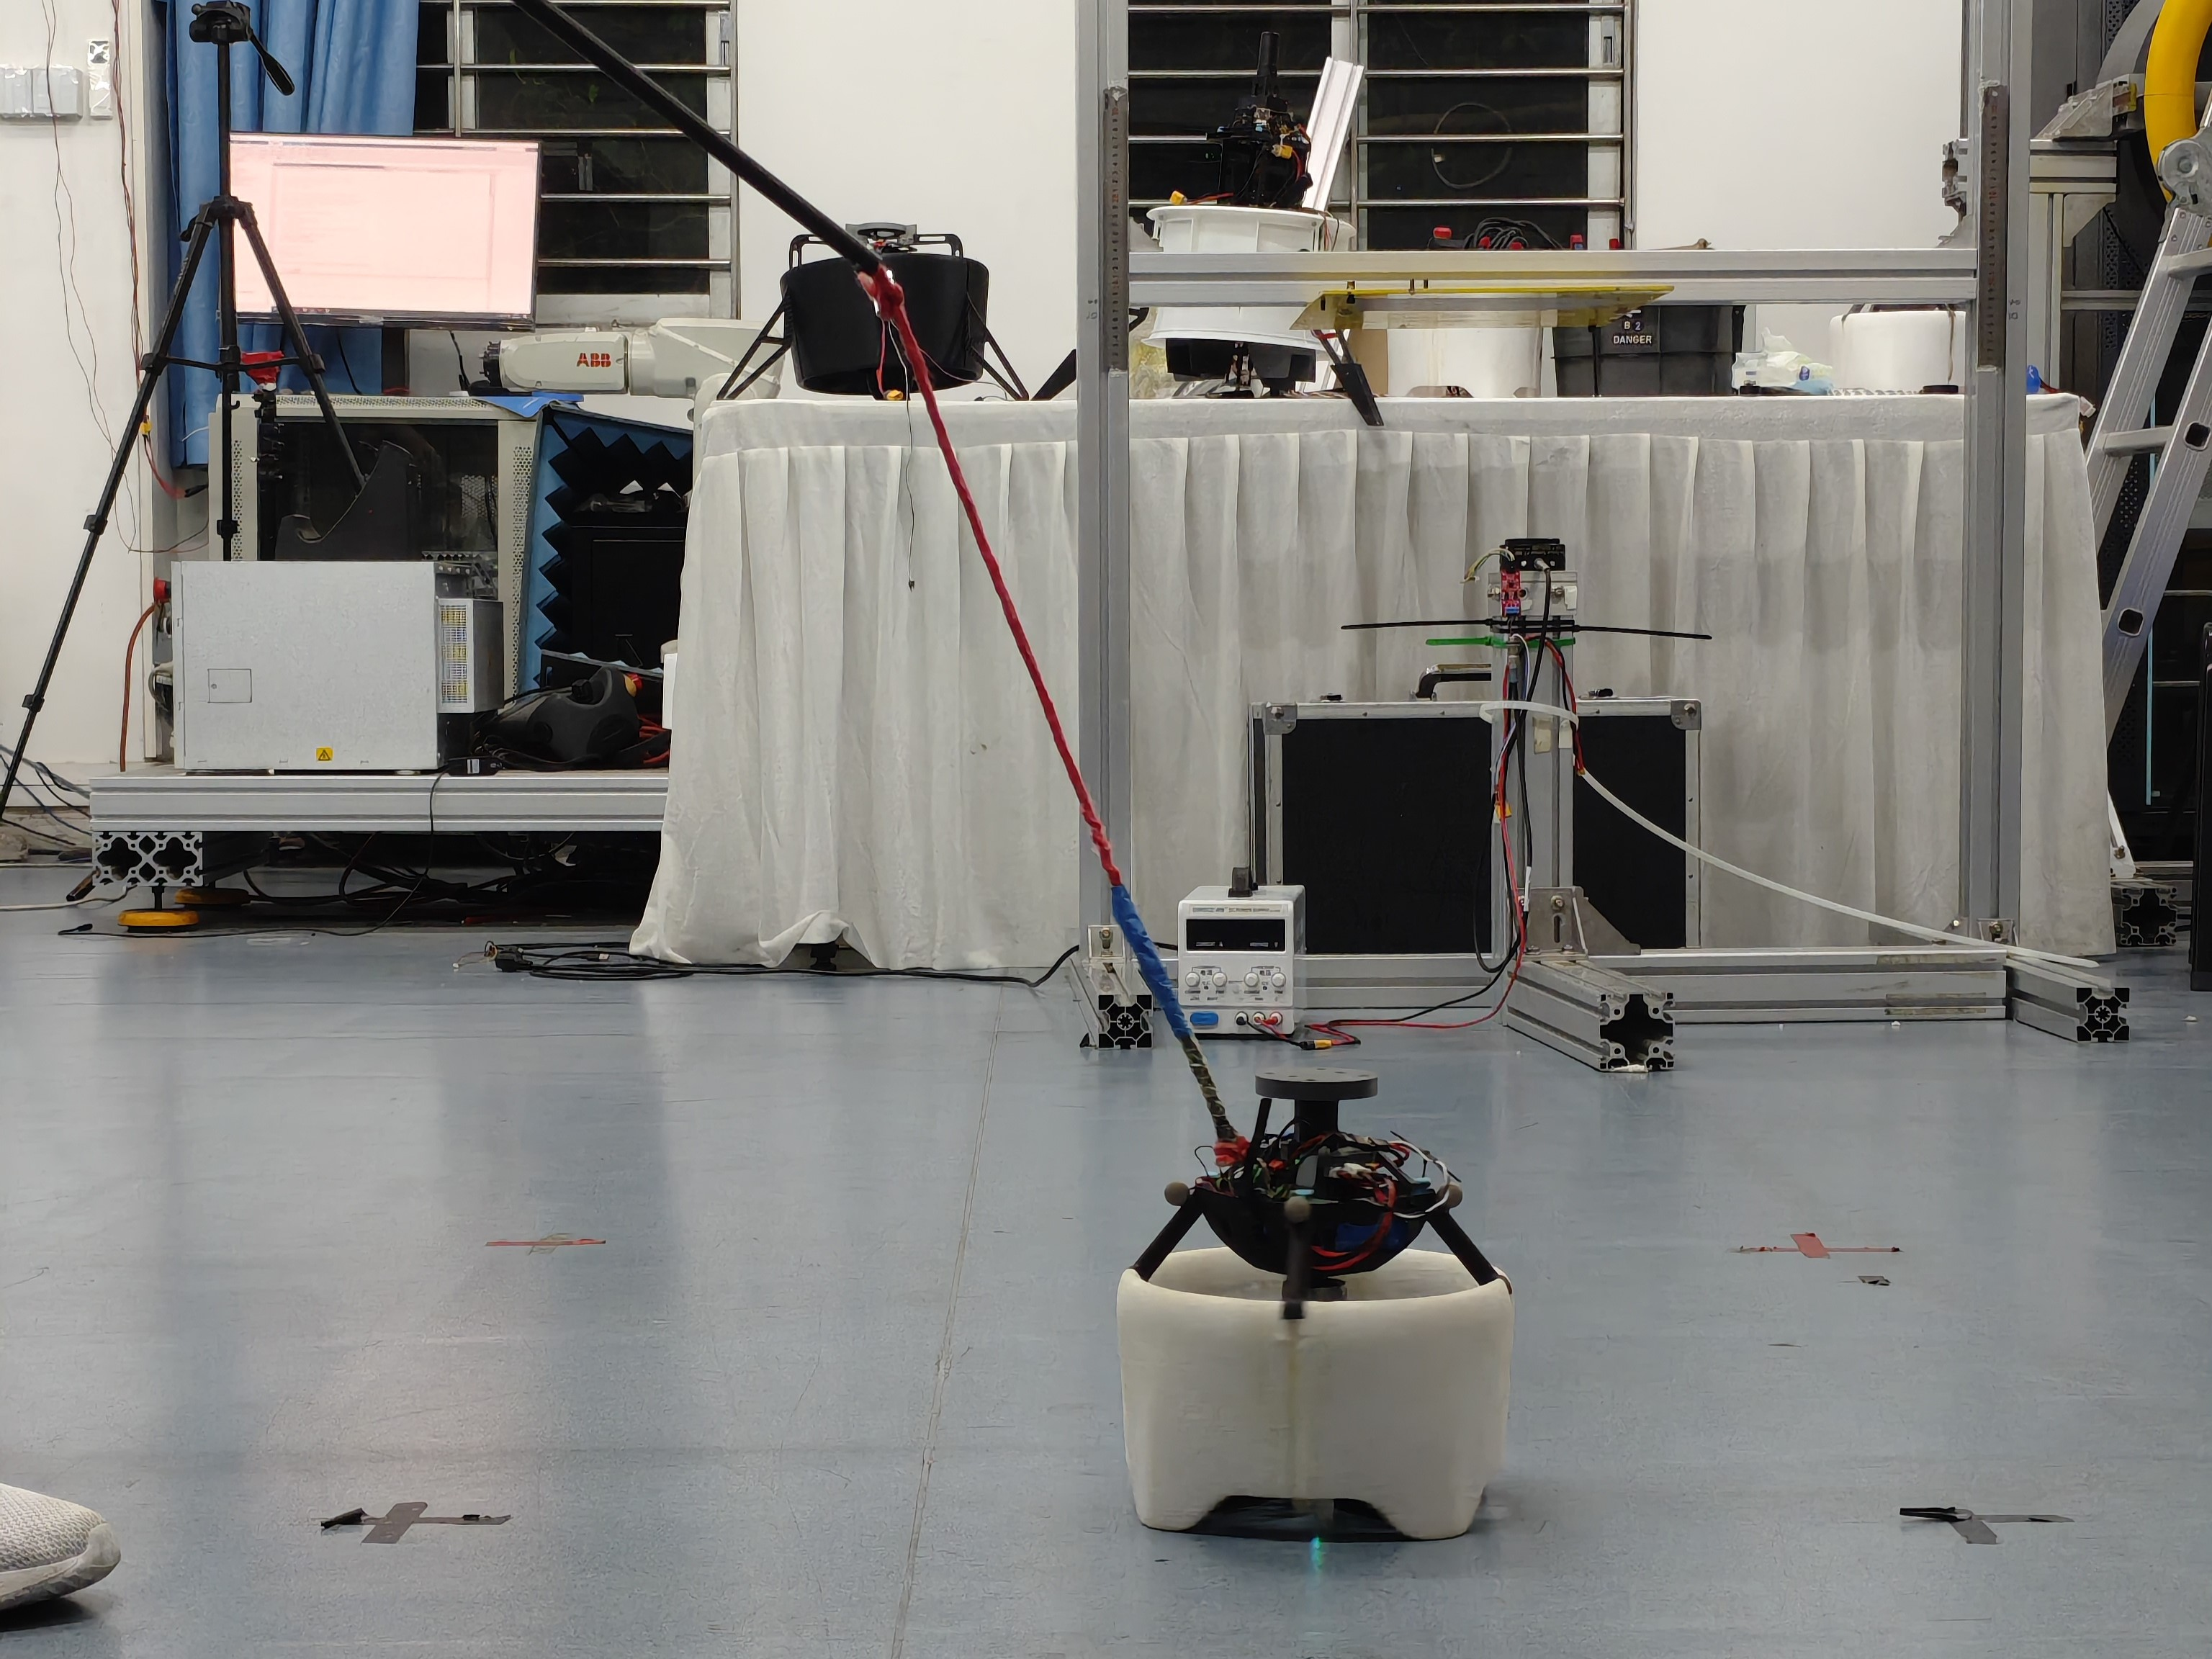
\includegraphics[height=0.20\textheight]{figure/chapter5/real_flght_scene_1.jpg}
        \caption*{(a)}
    \end{minipage}
    \hfill  % 产生弹性水平间距
    \begin{minipage}[b]{0.45\textwidth}
        \centering
        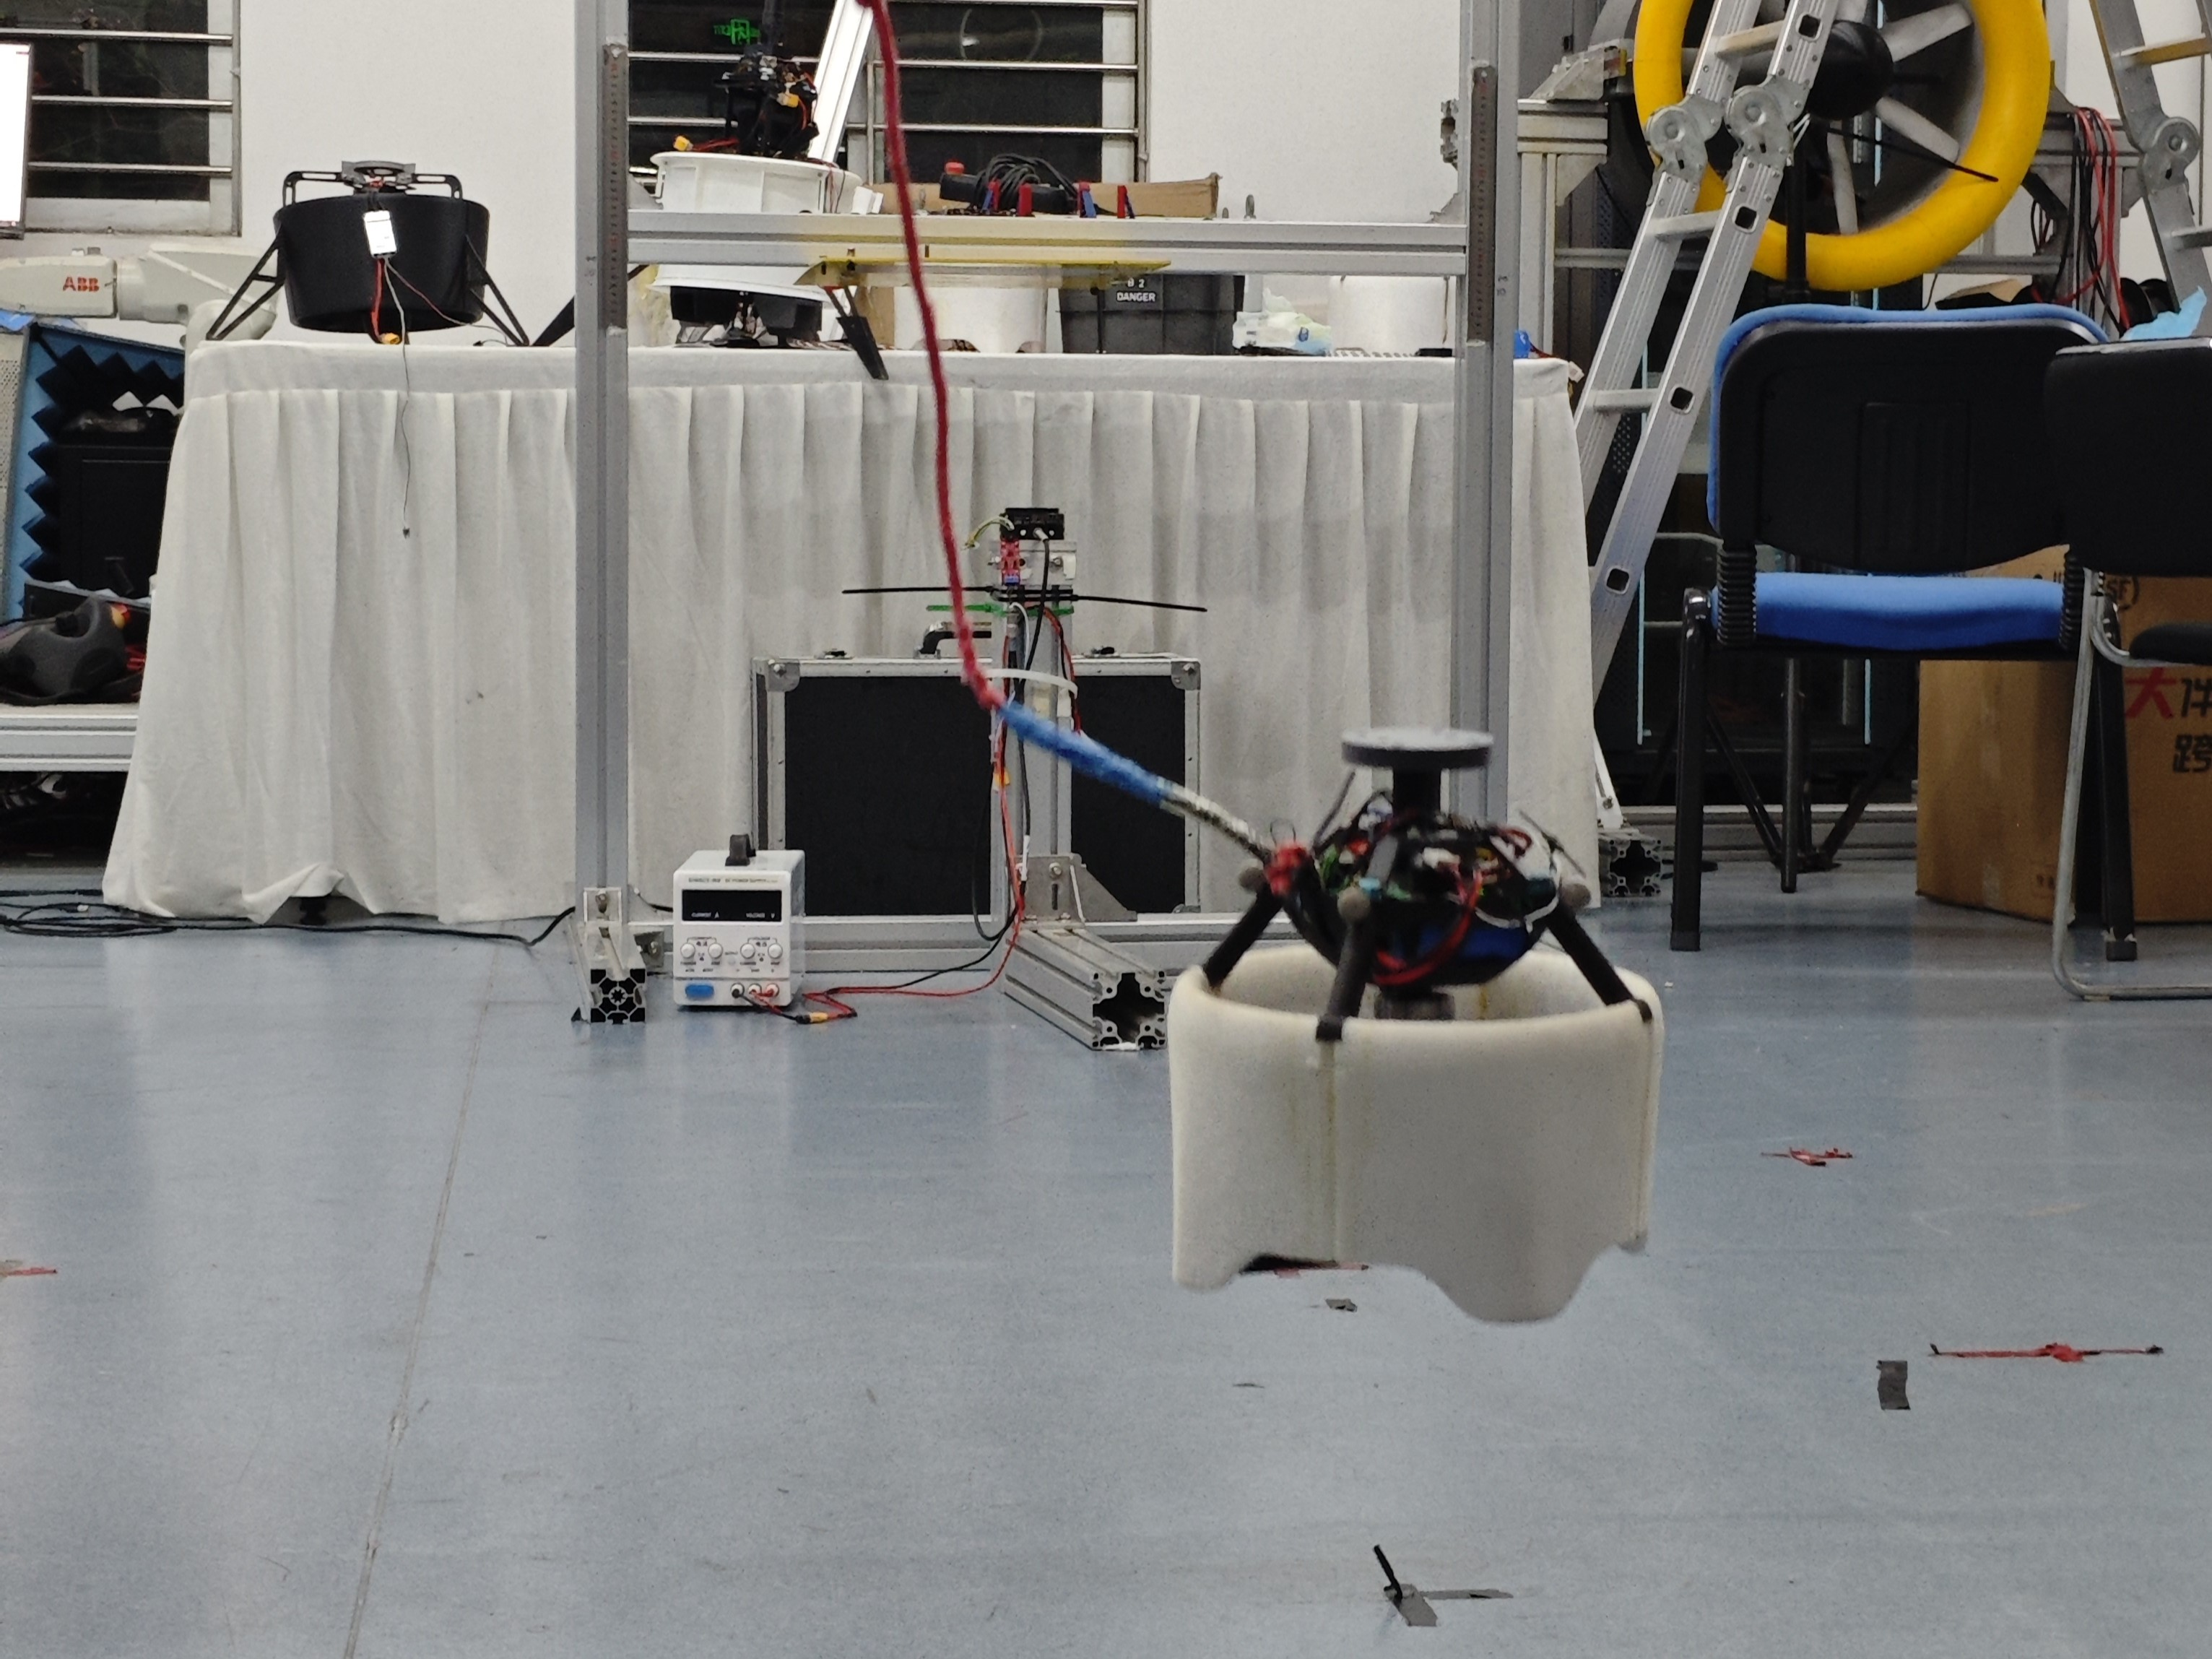
\includegraphics[height=0.20\textheight]{figure/chapter5/real_flght_scene_2.jpg}
        \caption*{(b)}
    \end{minipage}

    \vspace{0.5cm}

    \centering
    \begin{minipage}[b]{0.45\textwidth}
        \centering
        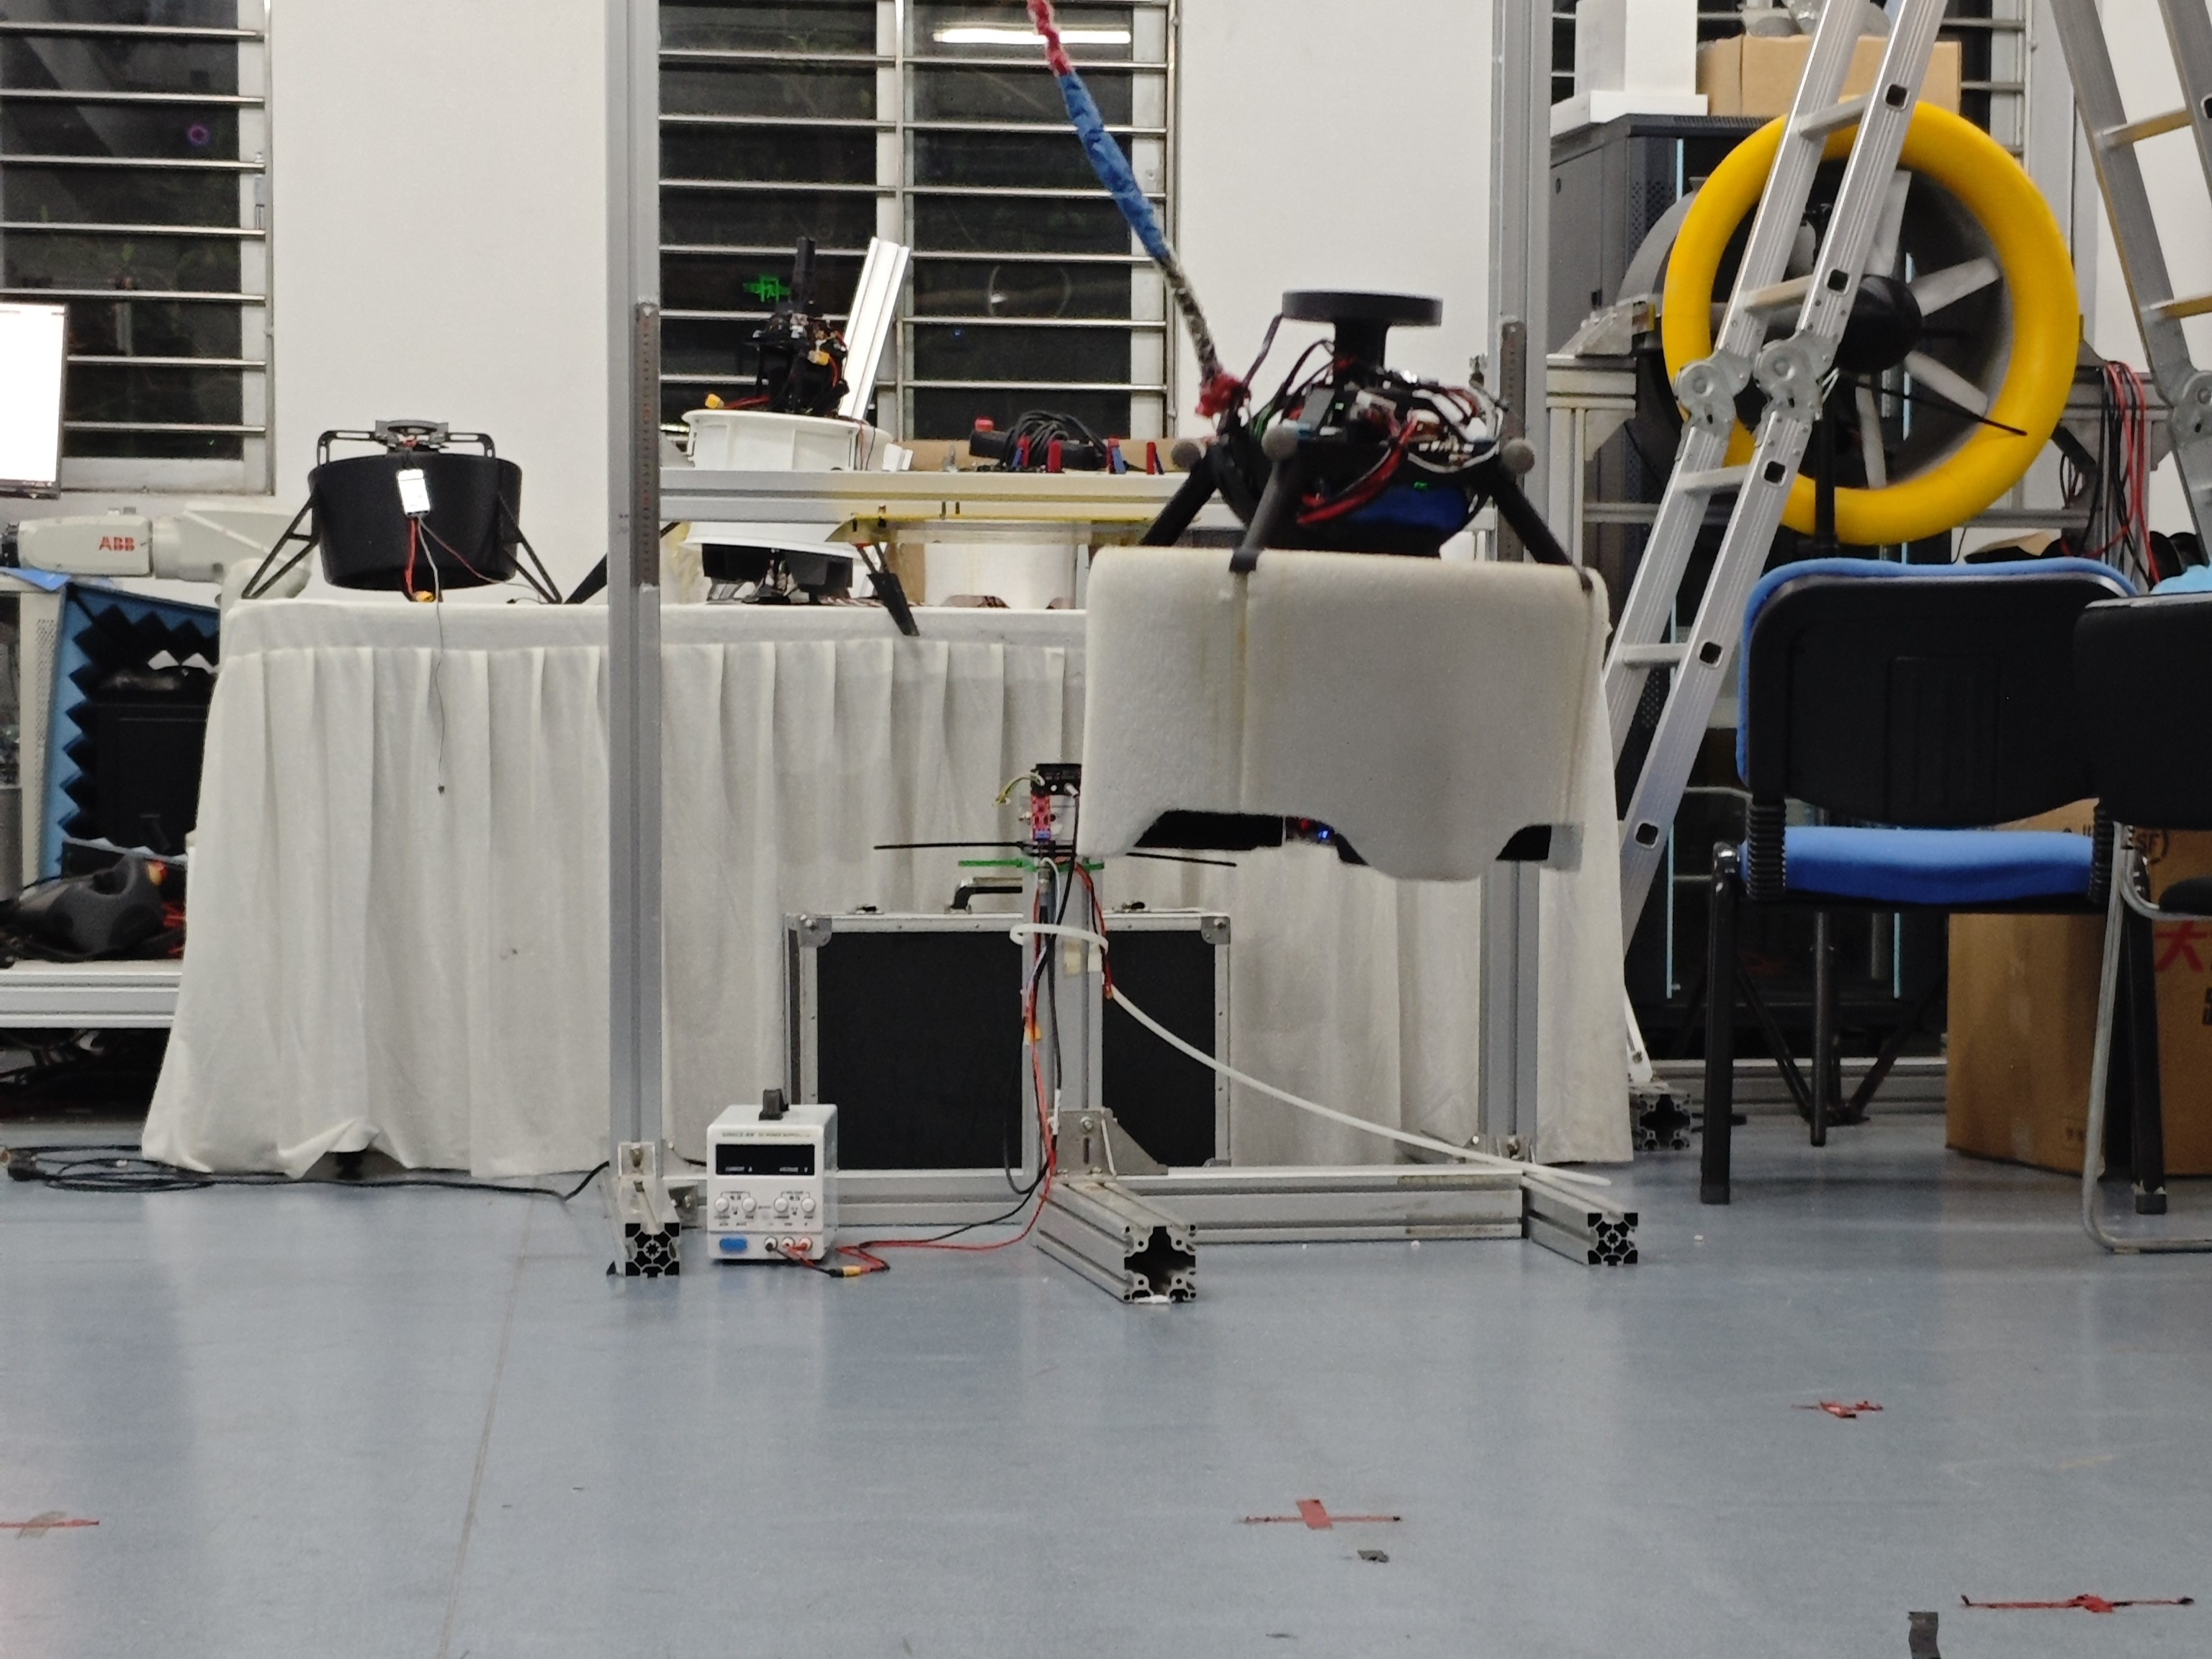
\includegraphics[height=0.20\textheight]{figure/chapter5/real_flght_scene_3.jpg}
        \caption*{(c)}
    \end{minipage}
    \hfill  % 产生弹性水平间距
    \begin{minipage}[b]{0.45\textwidth}
        \centering
        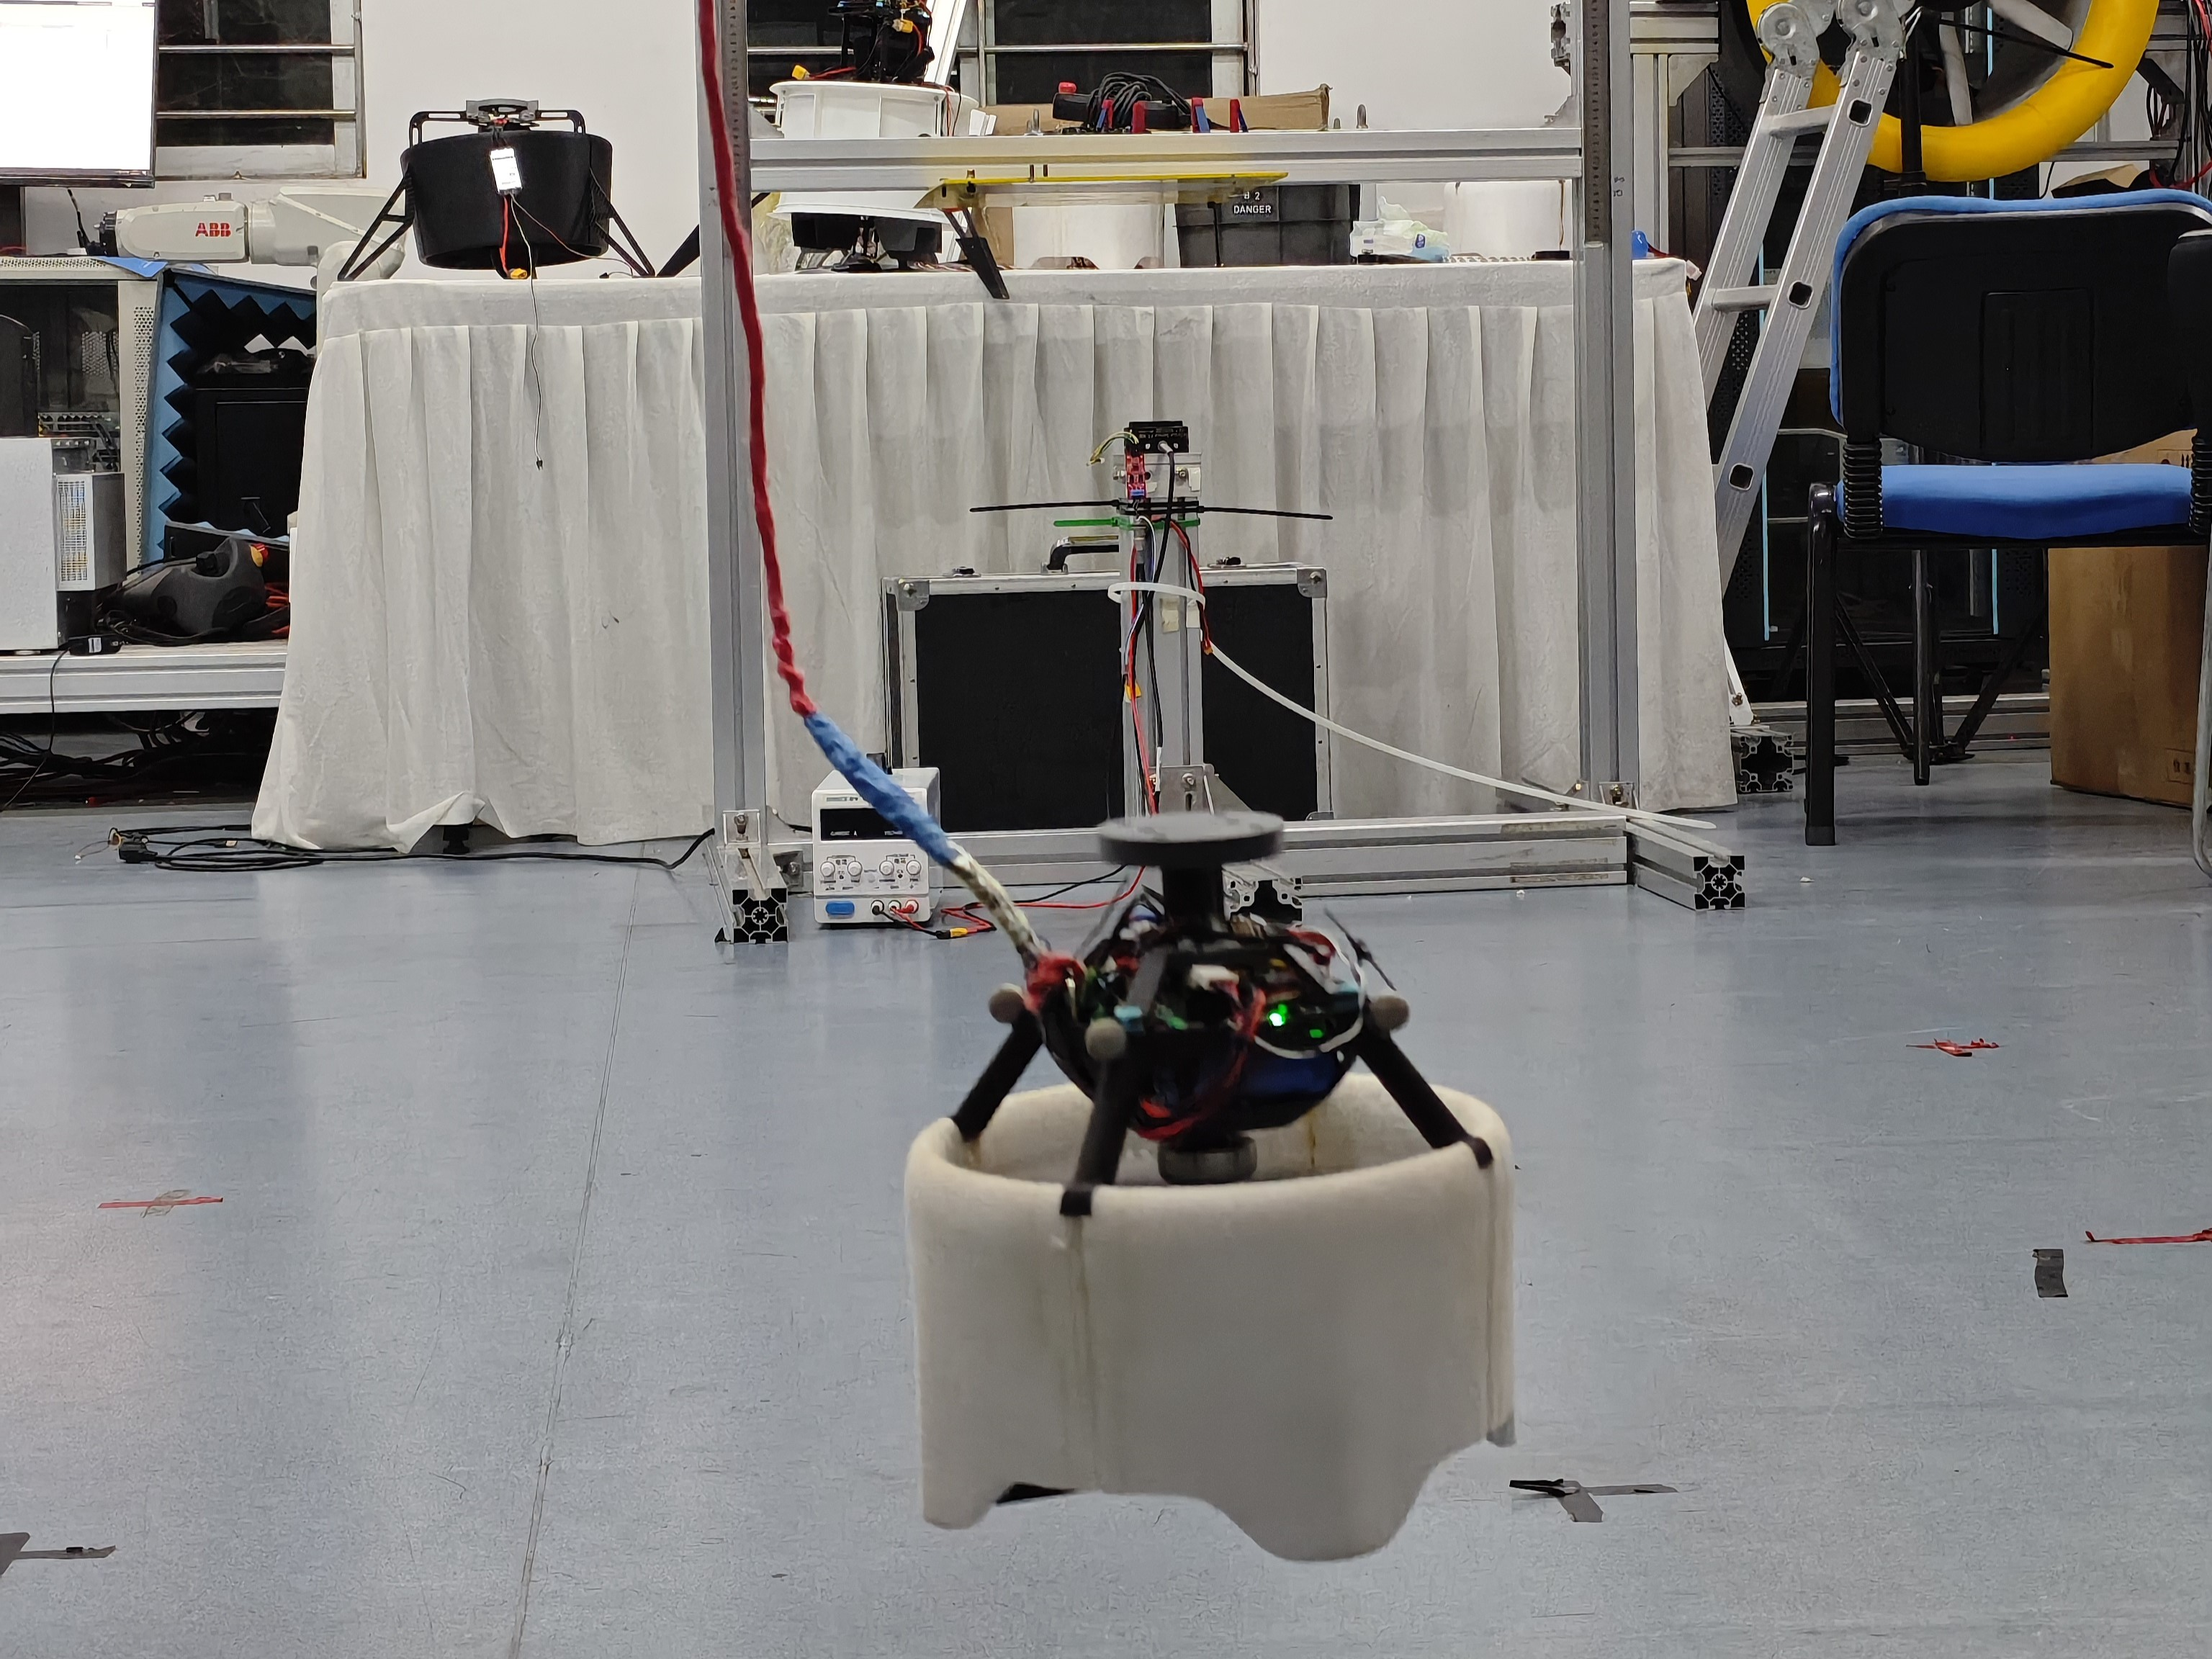
\includegraphics[height=0.20\textheight]{figure/chapter5/real_flght_scene_4.jpg}
        \caption*{(d)}
    \end{minipage}
    \caption{无人机地面效应抗扰控制实际飞行试验}
    \label{fig:anti_ge_flight}
\end{figure}

为保证系统在开放空间与近地面端具有一致的动态特性，两组实验均采用相同的串级PID控制器及其参数，且PID参数事先在开放空间下通过飞行试验整定完成。实验分为两组：第一组启用地面效应补偿算法（实验组），第二组不启用补偿算法（对照组）。通过对比无人机在近地面端的高度位置 \(p_z^e\) 阶跃响应以及不同高度下的偏航角 \(\psi\) 阶跃响应，分别验证推力补偿算法与控制舵面偏转角补偿算法的实际效果。

% 为保持系统能够在开放空间和近地面端能够有相同的动态特性，系统的PID控制器以及其参数在这两个环境下保持统一。

% 实验分两组进行，一组使用地面效应补偿算法，一组不使用。实验比较无人机在近地面端的高度位置$p_z^e$阶跃响应以及不同高度下的偏航角$\psi$阶跃响应以展示推力和控制舵面偏转角的地面效应补偿算法效果。

% 实验开始前，事先在开放空间下进行飞行试验并整定PID参数。
\subsection{高度位置阶跃响应实验步骤}
高度位置阶跃响应实验旨在验证推力补偿算法对地面效应下高度控制的改善效果。具体实验步骤如下：

1. 无人机上电后静置 \(10\,\mathrm{s}\)，待位姿估计滤波器收敛且动态捕捉系统数据稳定。

2. 向无人机发送起飞指令，无人机起飞并在高度 \(0.65\,\mathrm{m}\) 处保持稳定悬停。

3. 待无人机在空中稳定悬停 \(5\,\mathrm{s}\) 后，开始施加高度阶跃指令序列：依次给定期望高度为 \(0.3\,\mathrm{m}\) 和 \(0.1\,\mathrm{m}\)，分别对应无量纲高度 \(h/R \approx 3.37\) 与 \(h/R \approx 1.12\)，覆盖地效过渡区与强地效区。每个期望高度指令持续 \(5\,\mathrm{s}\)，并重复上述阶跃序列共三次，以验证算法的重复性与稳定性。

4. 飞行过程中，以 \(100\,\mathrm{Hz}\) 的采样频率记录以下数据：期望位置高度 \(p_{z,d}^e\)、实际位置高度 \(p_z^e\)、期望 \(Z\) 轴速度 \(v_{z,d}^e\)、实际 \(Z\) 轴速度 \(v_z^e\)、期望加速度 \(a_{z,d}^e\) 以及期望螺旋桨转速 \(\Omega_d\)，所有数据连同对应时间戳一并保存至机载 SD 卡。

5. 完成所有高度阶跃测试后，向无人机发送降落指令，结束本次实验。

6. 每组实验重复三至四次，以排除单次飞行中的偶然误差，保证实验结论的可靠性。

实验结束后，将 SD 卡中记录的数据导出至计算机进行离线处理与分析。通过对比实验组与对照组在不同高度阶跃指令下的高度跟踪误差、响应速度及稳态精度，定量评估推力补偿算法对近地面高度控制的改善效果。

% \subsection{高度位置阶跃响应实验步骤}
% 具体实验步骤如下
% 1. 无人机上电后静置10秒待位姿估计收敛，以及动态捕捉系统数据稳定。
% 2. 向无人机发送起飞指令，无人机起飞并在高度为0.65m处保持稳定
% 3. 待无人机在空中稳定悬停5s后，开始给定高度阶跃指令，轮流给定期望高度为0.3m，0.1m，给定高度后保持指令5s，反复执行3次。
% 4. 记录飞行过程中的期望位置高度，实际位置高度，期望z轴速度，实际z轴速度，期望加速度以及期望螺旋桨转速，并将这些数据以及对应的时间戳保存在SD卡中。
% 5. 向无人机发送降落指令。
% 6. 上述步骤每个实验重复三到四次。
\subsection{高度位置阶跃响应实验数据分析}

按照上述实验步骤完成飞行测试后，对采集到的高度位置与速度数据进行离线处理与分析。本小节通过对比未引入补偿与引入补偿两组实验的 $Z$ 轴高度 $p_z^e$ 跟随曲线和 $Z$ 轴速度 $v_z^e$ 跟随曲线，定量评估推力补偿算法对近地面高度控制的改善效果。

未引入地面效应补偿时，$Z$ 轴高度 $p_z^e$ 跟随曲线和速度 $v_z^e$ 跟随曲线分别如图\ref{fig:anti_height_cmp_p}和图\ref{fig:anti_height_cmp_v}所示；引入补偿后，相应的跟随曲线如图\ref{fig:anti_height_p}和图\ref{fig:anti_height_v}所示。

\begin{figure}[htbp]
    \centering
    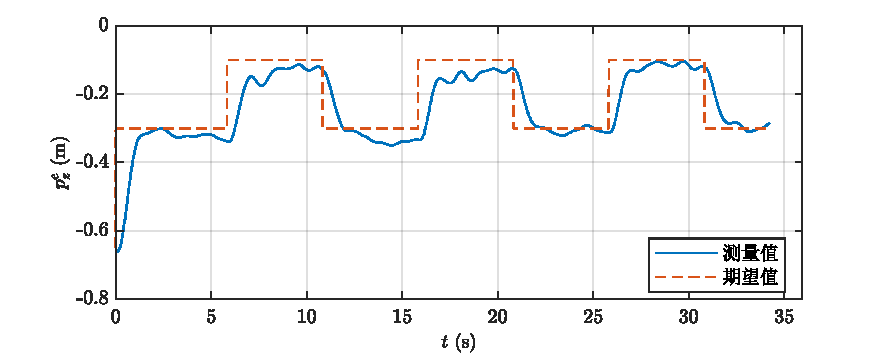
\includegraphics{matlab/ground_effect/pdf/anti_ge_height/anti_ge_height_cmp_pos.pdf}
    \caption{未引入补偿时 $Z$ 轴高度 $p_z^e$ 跟随曲线}
    \label{fig:anti_height_cmp_p}
\end{figure}

\begin{figure}[htbp]
    \centering
    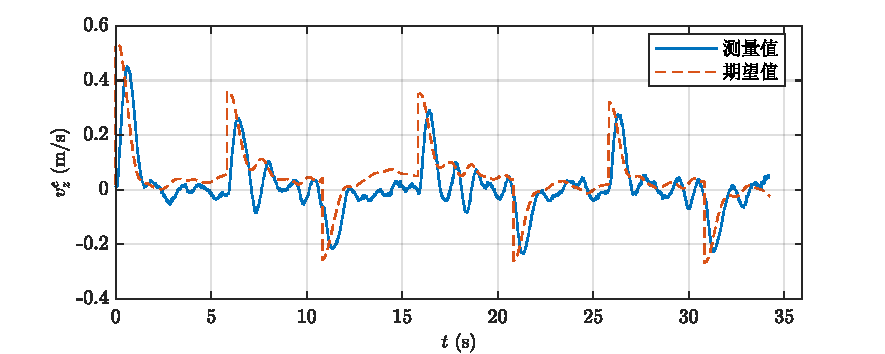
\includegraphics{matlab/ground_effect/pdf/anti_ge_height/anti_ge_height_cmp_vel.pdf}
    \caption{未引入补偿时 $Z$ 轴速度 $v_z^e$ 跟随曲线}
    \label{fig:anti_height_cmp_v}
\end{figure}

\begin{figure}[htbp]
    \centering
    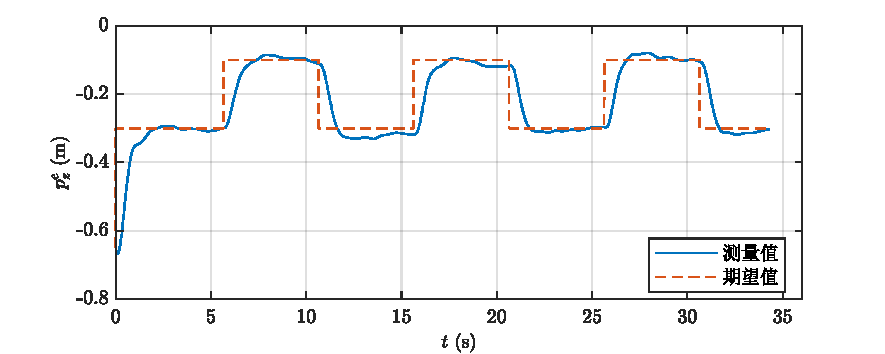
\includegraphics{matlab/ground_effect/pdf/anti_ge_height/anti_ge_height_pos.pdf}
    \caption{引入补偿后 $Z$ 轴高度 $p_z^e$ 跟随曲线}
    \label{fig:anti_height_p}
\end{figure}

\begin{figure}[htbp]
    \centering
    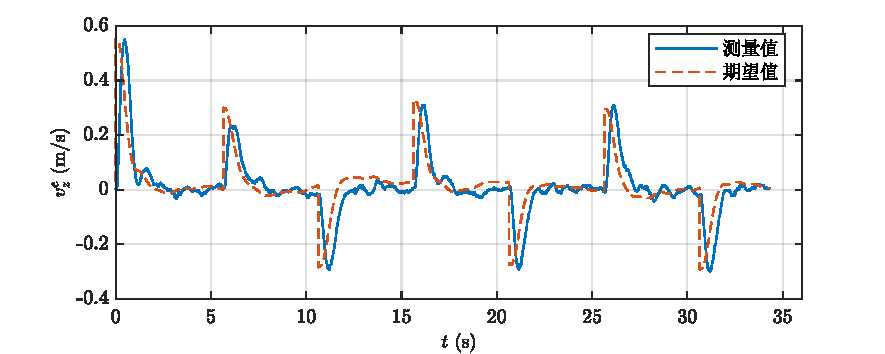
\includegraphics{matlab/ground_effect/pdf/anti_ge_height/anti_ge_height_vel.pdf}
    \caption{引入补偿后 $Z$ 轴速度 $v_z^e$ 跟随曲线}
    \label{fig:anti_height_v}
\end{figure}

从图中可以看出，实验开始后，无人机先由 $0.65\,\mathrm{m}$ 阶跃至 $0.3\,\mathrm{m}$，之后在 $0.3\,\mathrm{m}$ 与 $0.1\,\mathrm{m}$ 之间周期性地来回切换。其中 $0.3\,\mathrm{m}$ 对应弱地效区（$h/R \approx 3.4$），$0.1\,\mathrm{m}$ 对应强地效区（$h/R \approx 1.1$）。

由图\ref{fig:anti_height_cmp_p}可见，在 $t = 0\,\mathrm{s}$ 附近，无人机高度位置从 $0.65\,\mathrm{m}$ 向 $0.3\,\mathrm{m}$ 的阶跃响应中，高度位置跟踪较为平缓，未出现明显超调。这是由于 $0.3\,\mathrm{m}$ 处于弱地效区，地面效应对推力的增益尚不显著，在开放空间整定的 PID 参数仍能较好地维持系统稳定。相应地，由图\ref{fig:anti_height_cmp_v}可见，速度跟随曲线也表现良好，未出现明显超调，响应迅速。这说明在无地效区及弱地效范围内，原有 PID 参数具有足够的鲁棒性。

然而，当无人机在 $t \approx 6\,\mathrm{s}$ 处从 $0.3\,\mathrm{m}$ 阶跃下降至 $0.1\,\mathrm{m}$ 时，控制品质显著恶化。从图\ref{fig:anti_height_cmp_p}可以看出，实际高度虽然能够对阶跃指令做出响应，但难以收敛至稳态值，出现持续的振荡与稳态误差。同时，速度跟随曲线（图\ref{fig:anti_height_cmp_v}）呈现出明显的超调与多次振荡，在高度切换瞬间速度峰值远超期望值，且调节时间显著延长。

造成上述现象的根本原因在于：$0.1\,\mathrm{m}$ 处于强地效区，根据第四章辨识结果，该高度下涵道风扇的推力系数 $K_{TGE}$ 较无地效状态显著增大。在相同的螺旋桨转速指令下，实际产生的推力远大于控制器预期，导致高度下降过程中减速不足，甚至出现“触底反弹”式的振荡。此外，推力对转速变化的灵敏度增强，使得原本在开放空间整定的 PID 增益相对过高，进一步放大了系统的超调与振荡。速度环需要依赖积分项缓慢地降低转速指令以抵消多余推力，这一过程严重拖慢了系统响应，降低了起飞与降落阶段的安全性。

相比之下，引入地面效应补偿算法后，系统的近地面控制性能得到显著改善。从图\ref{fig:anti_height_p}可以看出，在 $t \approx 6\,\mathrm{s}$ 处从 $0.3\,\mathrm{m}$ 向 $0.1\,\mathrm{m}$ 的阶跃响应中，实际高度能够迅速、平滑地跟踪期望轨迹，两者高度贴合，稳态误差在 $2\,\mathrm{s}$ 内基本收敛至零，过渡过程平稳且无明显超调。更为重要的是，无人机在 $0.3\,\mathrm{m}$ 与 $0.1\,\mathrm{m}$ 两个高度上的动态表现高度一致，均展现出良好的跟踪性能，表明补偿算法有效消除了地面效应对推力特性的非线性调制，使得闭环系统在不同高度下具有一致的动态特性。

从速度跟随曲线（图\ref{fig:anti_height_v}）同样可以看出，引入补偿后速度环的超调与振荡现象基本消除，实际速度能够平稳地跟随期望速度曲线，稳态误差控制在可接受范围内，响应速度与无地效区相当。

高度位置阶跃响应实验结果表明：本文所设计的地面效应推力补偿算法能够有效克服强地效区推力增益带来的不利影响，显著改善近地面高度控制的稳态精度与动态品质，使无人机在 $0.1\,\mathrm{m}$ 与 $0.3\,\mathrm{m}$ 高度上展现出高度一致的动态特性，为安全起降与低空悬停提供了可靠保障。
% \subsection{高度位置阶跃响应实验数据分析}
% 经整理，实验数据如下。
% 未引入补偿时的$Z$轴高度$p_z^e$跟随曲线和$Z$轴速度$v_z^e$跟随曲线分别如图\ref{fig:anti_height_cmp_p}和图\ref{fig:anti_height_cmp_v}所示。引入补偿后的$Z$轴高度$p_z^e$跟随曲线和$Z$轴速度$v_z^e$跟随曲线分别如图\ref{fig:anti_height_p}和图\ref{fig:anti_height_v}所示。

% \begin{figure}[htbp]
%     \centering
%     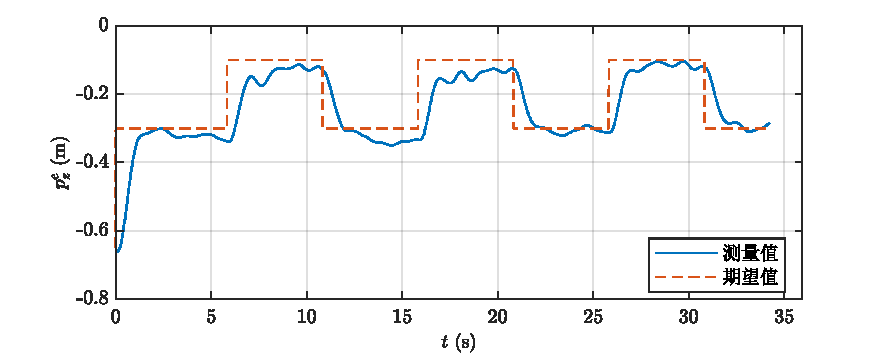
\includegraphics{matlab/ground_effect/pdf/anti_ge_height/anti_ge_height_cmp_pos.pdf}
%     \caption{未引入补偿时$Z$轴高度$p_z^e$跟随曲线}
%     \label{fig:anti_height_cmp_p}
% \end{figure}
% \begin{figure}[htbp]
%     \centering
%     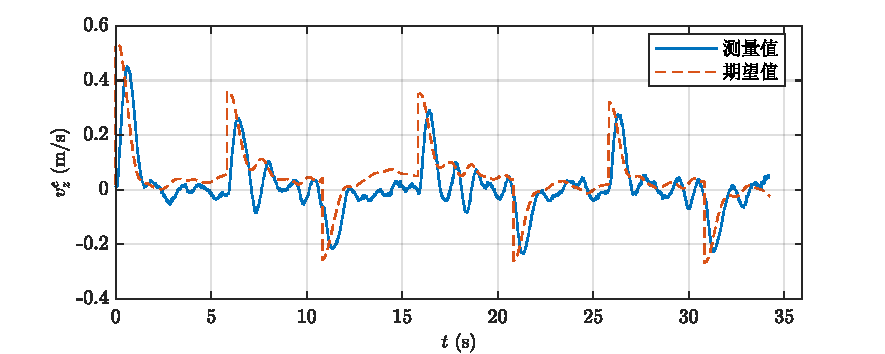
\includegraphics{matlab/ground_effect/pdf/anti_ge_height/anti_ge_height_cmp_vel.pdf}
%     \caption{未引入补偿时$Z$轴速度$v_z^e$跟随曲线}
%     \label{fig:anti_height_cmp_v}
% \end{figure}

% \begin{figure}[htbp]
%     \centering
%     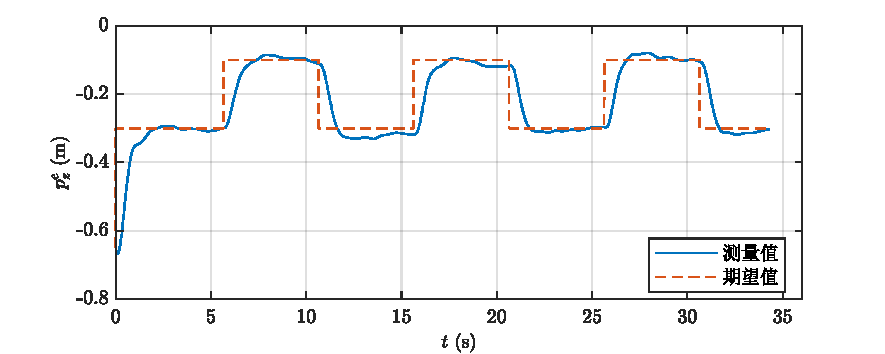
\includegraphics{matlab/ground_effect/pdf/anti_ge_height/anti_ge_height_pos.pdf}
%     \caption{引入补偿后$Z$轴高度$p_z^e$跟随曲线}
%     \label{fig:anti_height_p}
% \end{figure}
% \begin{figure}[htbp]
%     \centering
%     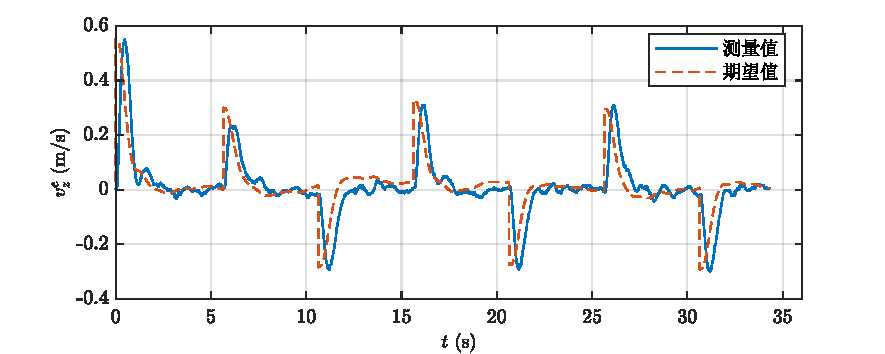
\includegraphics{matlab/ground_effect/pdf/anti_ge_height/anti_ge_height_vel.pdf}
%     \caption{引入补偿后$Z$轴速度$v_z^e$跟随曲线}
%     \label{fig:anti_height_v}
% \end{figure}

% 由图可见，实验开始时，给出从0.65m到0.3m的阶跃信号，此后周期性地产生从0.3m和0.1m之间来回切换的阶跃信号。

% 在未引入地面效应补偿时，由图\ref{fig:anti_height_cmp_p}可见，第0s时高度位置对于期望值从0.6m到0.3m的阶跃信号的跟随较为平缓，未出现超调现象，这是0.3m为弱地效区域，处于开放区域整定的PID参数能够在该位置较为良好地维持系统稳定。此时速度跟随也表现良好，未出现明显超调，且响应迅速。这说明在开放空间以及弱地效范围，该PID参数的有效性。

% 而第6s时从0.3m到0.1m的阶跃信号的位置跟随系统虽然能够对期望高度的阶跃信号做出响应，但控制品质较差。表现出难以收敛到稳态值的现象，此外速度跟随曲线也呈现出明显的超调震荡，并且在切换的时候，。这是由于0.1m的区域为强地效区，相同的螺旋桨转速下，推力相比开放空间更加明显，在该区域里，速度需要通过速度环PID控制器的积分项缓慢降低输出的螺旋桨转速。这种现象将大大降低无人机的起飞和降落安全性。

% 此外由于此时螺旋桨的推力系数$K_{TGE}$相比开放空间更大，因此，推力对螺旋桨转速变化的响应更加敏感。因此，使用相同的PID参数会输出动态变化更加明显的推力，从而令原有系统发生超调。

% 相比之下，加入地面效应补偿算法后，面对第6s时从0.3m到0.1m的阶跃信号，位置跟随曲线表现出了较为优异的控制性能。无人机的高度测量值能够迅速、平滑地追踪上期望轨迹。实际测量曲线与期望曲线保持高度贴合，稳态误差在2s内基本趋近于零，过渡过程平稳且快速。在0.3m和0.1m的表现较为一致。

% 此外，速度环的超调现象也基本消除，能够平稳地跟上目标曲线，并且不存在明显的稳态误差。

% 可见引入抗地面效应补偿后，在近地面端尤其是h=100mm时，高度的实际位置能够较为迅速且平缓地跟随期望位置，并且在h=100mm和h=300mm展现出较为一致的动态特性。


\subsection{偏航角阶跃响应实验步骤}
偏航角阶跃响应实验旨在验证舵面偏转力补偿算法在不同离地高度下对偏航通道控制效果的改善作用。由于偏航力矩完全由四个控制舵面的偏转力产生，且地面效应对舵面效率的衰减随高度变化显著，该实验能够直接反映 \(K_{cvGE}\) 补偿算法的有效性。具体实验步骤如下：

1. 无人机上电静置 \(10\,\mathrm{s}\) 待系统稳定，随后起飞到\(0.65\mathrm{m}\)待无人机稳定后，开始给无人机施加指令。

2. 令无人机依次悬停于两个个典型高度：\(0.20\,\mathrm{m}\)（地效过渡区）和 \(0.10\,\mathrm{m}\)（强地效区）。

3. 在每个固定高度上，待无人机悬停稳定 \(5\,\mathrm{s}\) 后，施加偏航角阶跃指令：期望偏航角 \(\psi_d\) 从当前值阶跃增加 \(30^\circ\)（即 \(\Delta\psi = 30^\circ\)），保持该指令 \(5\,\mathrm{s}\)，随后阶跃返回原角度，再保持 \(5\,\mathrm{s}\)。重复该阶跃序列三次。

4. 飞行过程中，以 \(100\,\mathrm{Hz}\) 的采样频率记录以下数据：期望偏航角 \(\psi_d\)、实际偏航角 \(\psi\)、期望偏航角速度 \(r_d\)、实际偏航角速度 \(r\)、四个舵面的期望偏转角 \(\delta_{i,d}\) 与实际偏转角 \(\delta_i\)，以及当前离地高度 \(h\)。所有数据连同时间戳保存至 SD 卡。

5. 完成所有高度下的偏航阶跃测试后，发送降落指令结束实验。每组高度工况重复三次。

\subsection{偏航角阶跃响应实验数据分析}
按照上述实验步骤完成飞行测试后，对采集到的偏航角与角速度数据进行离线处理与分析。本小节通过对比未引入补偿与引入补偿两组实验的偏航角 \(\psi\) 跟随曲线和 \(Z\) 轴角速度 \(r\) 跟随曲线，定量评估舵面偏转力补偿算法对近地面偏航通道控制性能的改善效果。

在强地效区（\(h = 100\,\mathrm{mm}\)，对应 \(h/R = 0.56\)）和地效过渡区（\(h = 200\,\mathrm{mm}\)，对应 \(h/R = 1.12\)）的偏航角与角速度跟随曲线分别如图\ref{fig:anti_ge_yaw_100mm_yaw}和图\ref{fig:anti_ge_yaw_200mm_yaw}所示。需要说明的是，实验开始时，无人机首先从无地效高度 \(0.65\,\mathrm{m}\) 快速下降至指定的近地面测试高度。由于螺旋桨转速的突变，涵道出口气流状态发生剧烈变化，导致偏航轴在 \(t \approx 0\,\mathrm{s}\) 时刻受到较大的初始扰动，因此各子图中均可见短暂的初始波动，随后系统迅速收敛至稳定状态。

% 按照上述实验步骤完成飞行测试后，对采集到的偏航角和角速度数据进行离线处理与分析。本小节通过对比未引入补偿与引入补偿两组实验的 偏航角 $\psi$ 跟随曲线和 $Z$ 轴速度 $r$ 跟随曲线，定量评估推力补偿算法对近地面姿态控制的改善效果。

% 高度为100mm时和高度为200mm时，偏航角$\psi$和角速度$r$的跟随曲线分别如图\ref{fig:anti_ge_yaw_100mm_yaw}和图\ref{fig:anti_ge_yaw_200mm_yaw}所示。

\begin{figure}[htbp]
    \begin{minipage}{1.0\textwidth}
        \centering
        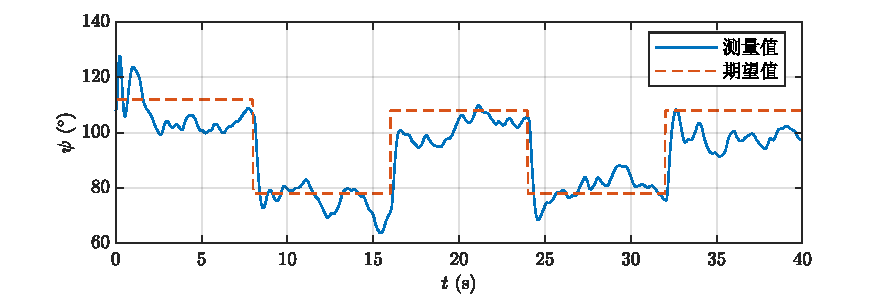
\includegraphics{matlab/ground_effect/pdf/anti_ge_yaw/anti_ge_yaw_100mm_cmp_yaw.pdf}
        \caption*{(a)未补偿时偏航角$\psi$跟随曲线}
    \end{minipage}
    \vspace{0.3cm}
    \begin{minipage}{1.0\textwidth}
        \centering
        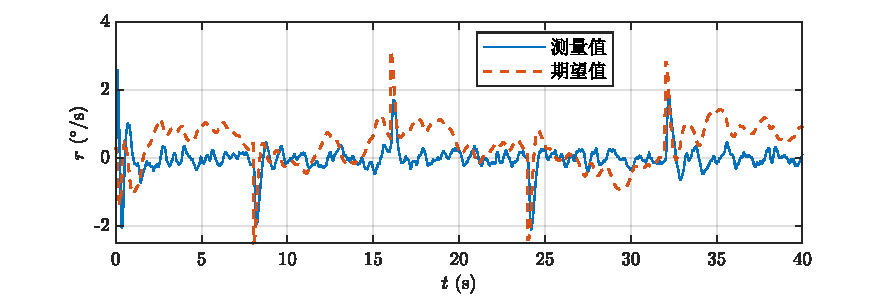
\includegraphics{matlab/ground_effect/pdf/anti_ge_yaw/anti_ge_yaw_100mm_cmp_gyro_z.pdf}
        \caption*{(b)未补偿时角速度$r$跟随曲线}
    \end{minipage}
    \vspace{0.3cm}
    \begin{minipage}{1.0\textwidth}
        \centering
        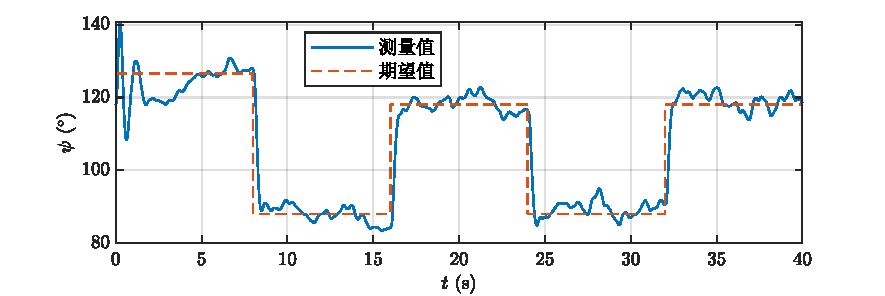
\includegraphics{matlab/ground_effect/pdf/anti_ge_yaw/anti_ge_yaw_100mm_yaw.pdf}
        \caption*{(c)补偿后偏航角$\psi$跟随曲线}
    \end{minipage}
    \vspace{0.3cm}
    \begin{minipage}{1.0\textwidth}
        \centering
        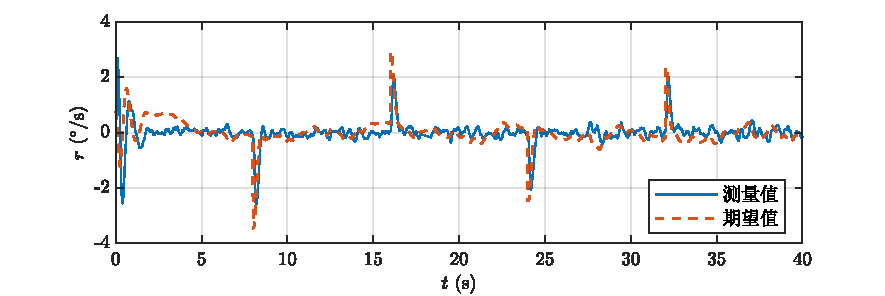
\includegraphics{matlab/ground_effect/pdf/anti_ge_yaw/anti_ge_yaw_100mm_gyro_z.pdf}
        \caption*{(d)补偿后角速度$r$跟随曲线}
    \end{minipage}
    \caption{实际飞行试验$h/R = 0.56$时偏航角$\psi$和角速度$r$跟随曲线}
    \label{fig:anti_ge_yaw_100mm_yaw}
\end{figure}

\begin{figure}[htbp]
    \begin{minipage}{1.0\textwidth}
        \centering
        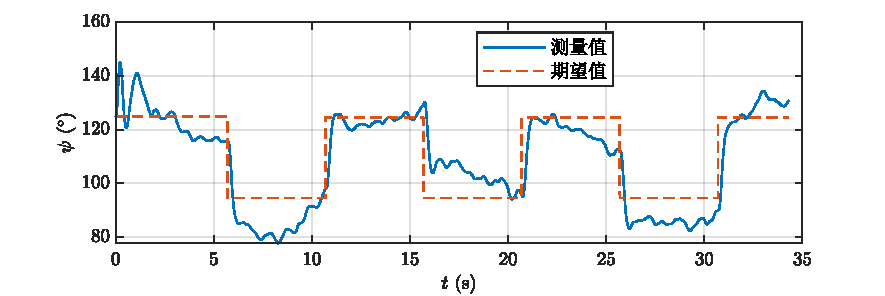
\includegraphics{matlab/ground_effect/pdf/anti_ge_yaw/anti_ge_yaw_200mm_cmp_yaw.pdf}
        \caption*{(a)未补偿时偏航角$\psi$跟随曲线}
    \end{minipage}
    \vspace{0.3cm}
    \begin{minipage}{1.0\textwidth}
        \centering
        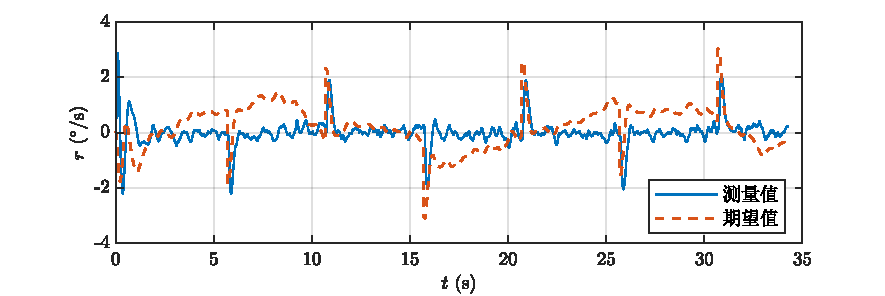
\includegraphics{matlab/ground_effect/pdf/anti_ge_yaw/anti_ge_yaw_200mm_cmp_gyro_z.pdf}
        \caption*{(b)未补偿时角速度$r$跟随曲线}
    \end{minipage}
    \vspace{0.3cm}
    \begin{minipage}{1.0\textwidth}
        \centering
        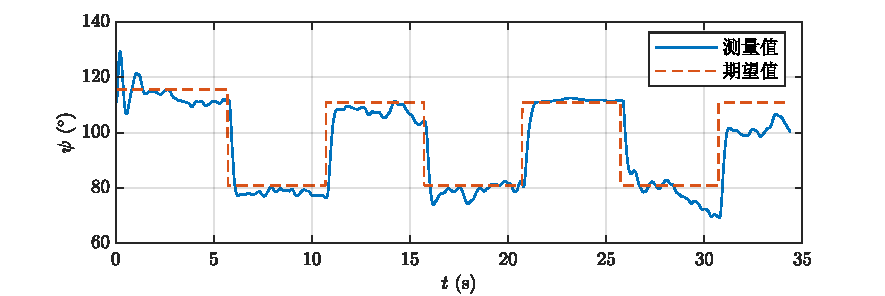
\includegraphics{matlab/ground_effect/pdf/anti_ge_yaw/anti_ge_yaw_200mm_yaw.pdf}
        \caption*{(c)补偿后偏航角$\psi$跟随曲线}
    \end{minipage}
    \vspace{0.3cm}
    \begin{minipage}{1.0\textwidth}
        \centering
        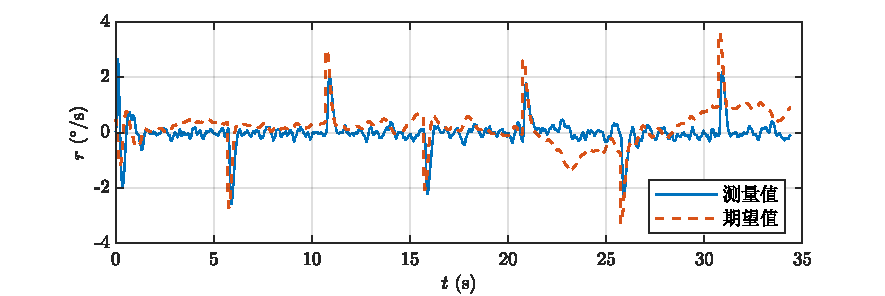
\includegraphics{matlab/ground_effect/pdf/anti_ge_yaw/anti_ge_yaw_200mm_gyro_z.pdf}
        \caption*{(d)补偿后角速度$r$跟随曲线}
    \end{minipage}
    \caption{实际飞行试验$h/R = 1.12$时偏航角$\psi$和角速度$r$跟随曲线}
    \label{fig:anti_ge_yaw_200mm_yaw}
\end{figure}

从图\ref{fig:anti_ge_yaw_100mm_yaw}(a)和图\ref{fig:anti_ge_yaw_200mm_yaw}(a)可以看出，在未引入舵面偏转力补偿的情况下，无人机虽然能够对 \(30^\circ\) 的偏航角阶跃指令做出响应，但控制品质较差，主要体现在以下两个方面：

其一，姿态抗扰动能力不足。在初始扰动阶段（\(t \approx 0\,\mathrm{s}\)），偏航角出现明显的瞬时偏差，且收敛速度较慢，需要约 \(2\,\mathrm{s}\) 才能基本回到指令值附近。在随后的阶跃响应过程中，实际偏航角与期望曲线之间存在持续的稳态偏差，尤其在 \(h = 100\,\mathrm{mm}\) 的强地效区，稳态误差达到 \(5^\circ\) 以上，调节时间超过 \(3\,\mathrm{s}\)。

其二，角速度跟踪响应滞后。从角速度曲线（图\ref{fig:anti_ge_yaw_100mm_yaw}(b)和图\ref{fig:anti_ge_yaw_200mm_yaw}(b)）可见，当偏航角误差出现时，角速度难以迅速响应并产生足够的反向角速度来抑制误差。在阶跃指令发出后，角速度上升缓慢，峰值角速度明显低于期望值，且存在多次振荡。这说明在近地面区域，由于地面对气流的约束与阻塞效应，控制舵面的偏转力系数 \(K_{cvGE}\) 显著衰减，导致相同舵面偏转角下产生的控制力矩大幅降低。角速度环需要更长的积分作用来累积足够的控制量，从而使响应变慢、超调增大。

相比之下，引入舵面偏转力补偿算法后，系统在近地面的偏航控制性能得到显著改善。从图\ref{fig:anti_ge_yaw_100mm_yaw}(c)和图\ref{fig:anti_ge_yaw_200mm_yaw}(c)可以看出，补偿后的偏航角能够迅速、平滑地跟踪期望轨迹，实际测量曲线与期望曲线高度贴合。在阶跃指令发出后，偏航角以近似一阶系统的响应形式平滑过渡，无超调，稳态误差在 \(0.5\,\mathrm{s}\) 内基本收敛至零。更为重要的是，无人机在 \(h = 100\,\mathrm{mm}\) 与 \(h = 200\,\mathrm{mm}\) 两个高度上的偏航动态表现高度一致，均展现出快速、准确的跟踪能力。

从角速度跟随曲线（图\ref{fig:anti_ge_yaw_100mm_yaw}(d)和图\ref{fig:anti_ge_yaw_200mm_yaw}(d)）同样可以看出，补偿后的角速度环能够快速响应误差信号，峰值角速度与期望值基本一致，且无明显振荡或长时间延迟。这表明通过动态更新控制效率矩阵 \(\boldsymbol{B}_{GE}\) 中的 \(K_{cvGE}\) 系数，控制分配模块能够准确补偿地面效应造成的舵面效率衰减，使得实际产生的偏航力矩与控制器期望值保持一致。

综合上述分析，偏航角阶跃响应实验结果表明：本文所设计的舵面偏转力补偿算法能够有效克服地面效应对偏航通道的不利影响，显著提升近地面姿态控制的响应速度与稳态精度。引入补偿后，无人机在 \(h = 100\,\mathrm{mm}\) 与 \(h = 200\,\mathrm{mm}\) 两个高度上展现出高度一致的动态特性，验证了补偿模型在不同地效强度下的有效性与鲁棒性。
% 由图可见，实验开始时，由于高度先从0.65m骤降到实验条件指定的近地面高度，受螺旋桨转速突变的影响，偏航轴会受到较大的扰动，因此在各组实验曲线上会呈现出在第0s存在扰动，然后迅速收敛。

% 在未引入地面效应补偿时，由图可见，面对30度的阶跃信号的偏航角跟随系统虽然能够对期望高度的阶跃信号做出响应，但控制品质较差。
% 主要表现无人机姿态角抗扰动性能较差，控制响应相对较慢。
% 在出现扰动后，Z轴角速度难以迅速跟随该误差，存在误差收敛慢的现象。
% 这是在0.1m和0.2m区域存在较强的气流扰动，且控制舵面的控制效果下降，面对近地面处的复杂气流扰动，对无人机的产生难以预测的力矩。与此同时，由于地面对气流的约束作用，导致系统的角速度增益下降，使角速度难以跟随。

% 相比之下，加入地面效应补偿算法后，面对30度偏航角阶跃信号，位置跟随曲线表现出了较为优异的控制性能。无人机的偏航角能够迅速、平滑地追踪上期望轨迹。实际测量曲线与期望曲线保持高度贴合，稳态误差在0.5s内基本趋近于零，过渡过程平稳且快速。并且在0.2m和0.1m的表现较为一致。

% 此外，角速度环基本上能够快速目标曲线，并且不存在明显长时间的误差。

% 可见引入抗地面效应补偿后，在近地面端尤其是h=100mm时，偏航角的能够较为迅速且平缓地跟随期望偏航角，并且在h=0.1m和h=0.2m展现出较为一致的动态特性。

本小节针对涵道式无人机近地面飞行时的地面效应扰动问题，设计了基于动态补偿的抗扰控制方法。通过实时更新控制效率矩阵中的推力系数 \(K_{TGE}\) 与舵面偏转力系数 \(K_{cvGE}\)，在控制分配环节实现了对地效影响的精确补偿。静态台架实验表明，补偿后推力与力矩的稳态误差分别控制在 \(3\%\) 与 \(10\%\) 以内。实飞验证进一步证明，引入补偿后无人机在强地效区的高度与偏航角跟踪性能显著提升，稳态误差快速收敛且动态品质一致。所提方法有效抑制了地面效应对飞行控制的不利影响，为涵道式无人机安全起降与低空悬停提供了可靠保障。

\section{非线性动态逆控制器}

前文重点解决了涵道式无人机在近地面飞行时由地面效应引起的执行器效益变化问题。然而，当无人机在开放环境中执行大机动、大迎角飞行或遭遇阵风扰动时，涵道风扇及控制舵面所受到的气动力与力矩呈现出强烈的非线性耦合特性。具体而言，涵道风扇的侧向力、拉力随迎角与前进比的变化具有明显的非线性依赖关系，陀螺力矩与反扭矩襟翼的平衡效果亦随飞行状态而改变。这些非线性气动特性难以通过简单的线性控制器实现精确补偿，若仍采用PID控制结构，往往会导致模型失配、控制精度下降，甚至在极端工况下引发系统失稳。

针对上述问题，非线性控制方法成为提升涵道式无人机全包线飞行品质的必然选择。目前学术界广泛采用的非线性控制策略包括反步控制、滑模控制、模型预测控制以及非线性动态逆控制等。其中，增量式非线性动态逆控制（Incremental Nonlinear Dynamic Inversion, INDI）因其对模型误差和外部扰动具有较强鲁棒性而受到关注\cite{Cheng2024INDI}。然而，INDI控制器依赖于高带宽的角加速度反馈，且对传感器噪声较为敏感，而单螺旋桨涵道式无人机的震动较大，陀螺仪测量值差分计算角加速度引入的噪声难以被忽略。相比之下，在系统精确模型进行反馈线性化已经被准确估计的前提下，非线性动态逆控制（Nonlinear Dynamic Inversion, NDI）能够将原始非线性系统映射为期望的线性解耦形式，具有响应速度快、控制精度高、结构清晰等优点。

由于本文已通过第二章推导出该无人机的动态，且第三章的在线参数辨识获得了该模型的气动参数，具备部署NDI控制器的先验条件，因此本小节将设计NDI控制器，并与INDI控制器的控制效果进行比较验证。

\subsection{NDI控制器介绍}
\label{sec:NDI_intro}

非线性动态逆控制是一种基于反馈线性化思想的非线性控制方法，其核心思路是：通过对被控对象的动力学模型求逆，构造一个伪线性系统，从而将复杂的非线性控制问题转化为线性系统的综合问题。具体而言，对于一类输入仿射的非线性系统，NDI控制律通过引入与系统非线性部分相反的项，直接抵消原系统的非线性特性，使闭环系统呈现出期望的线性动态行为。该方法在模型精确已知的前提下，能够实现大范围内的解耦与线性化，具有响应速度快、稳态精度高的优点。

针对本文所研究的涵道式无人机，NDI控制器的设计以姿态控制为例进行阐述。选取无人机的姿态角（滚转角 \(\varphi\)、俯仰角 \(\theta\)、偏航角 \(\psi\)）作为被控输出。首先，根据第二章建立的动力学模型，推导姿态角加速度与控制输入（即控制舵面产生的力矩 \(\boldsymbol{M}_{cv}^b\)）之间的解析关系。

由式\eqref{eq:d_eular}可知：
\begin{equation}
    \dot{\boldsymbol{\eta}} = \boldsymbol{Q} \cdot \boldsymbol{\omega}^b.
    \label{eq:Q_ref}
\end{equation}

式\eqref{eq:Q_ref}对时间求导可得：
\begin{equation}
    \ddot{\boldsymbol{\eta}} = \dot{\boldsymbol{Q}} \cdot \boldsymbol{\omega}^b + \boldsymbol{Q} \cdot \dot{\boldsymbol{\omega}}^b,
    \label{eq:ddot_eta}
\end{equation}
其中\(\dot{\boldsymbol{\omega}}^b\)是角速度对时间的导数，在式\eqref{eq:d_omega}已给出，\(\dot{\boldsymbol{Q}}\)是矩阵\(\boldsymbol{Q}\)对时间的导数，可由下式给出：
\begin{equation}
    \dot{\boldsymbol{Q}} = 
    \begin{bmatrix}
        0 & \dot{Q}_{12} & \dot{Q}_{13} \\
        0 & \dot{Q}_{22} & \dot{Q}_{23} \\
        0 & \dot{Q}_{32} & \dot{Q}_{33}
    \end{bmatrix},
\end{equation}
且各元素的定义如下：
\begin{equation}
    \begin{aligned}
        \dot{Q}_{12} =& \dot{\varphi}\cos\varphi\tan\theta + \dot{\theta}\sin\varphi\sec^2\theta, \\
        \dot{Q}_{13} =& -\dot{\varphi}\sin\varphi\tan\theta + \dot{\theta}\cos\varphi\sec^2\theta, \\
        \dot{Q}_{22} =& -\dot{\varphi}\sin\varphi, \\
        \dot{Q}_{23} =& -\dot{\varphi}\cos\varphi, \\
        \dot{Q}_{32} =& \dot{\varphi}\cos\varphi\sec\theta + \dot{\theta}\sin\varphi\sec\theta\tan\theta, \\
        \dot{Q}_{33} =& -\dot{\varphi}\sin\varphi\sec\theta + \dot{\theta}\cos\varphi\sec\theta\tan\theta.
    \end{aligned}
\end{equation}

将式\eqref{eq:d_omega}代入式\eqref{eq:ddot_eta}中，可得：
\begin{equation}
    \ddot{\boldsymbol{\eta}} = \dot{\boldsymbol{Q}} \cdot \boldsymbol{\omega}^b + \boldsymbol{Q} \cdot \boldsymbol{J}^{-1}(\boldsymbol{M}^b - \boldsymbol{\omega}^b\times(\boldsymbol{J}\cdot\boldsymbol{\omega}^b)).
    \label{eq:ddot_eta_ref}
\end{equation}

并根据式\eqref{eq:total_effort}将\(\boldsymbol{M}^b\)展开，可得：
\begin{equation}
    \ddot{\boldsymbol{\eta}} = \dot{\boldsymbol{Q}} \cdot \boldsymbol{\omega}^b + \boldsymbol{Q} \cdot \boldsymbol{J}^{-1}(\boldsymbol{M}_{df}^b + \boldsymbol{M}_{fan}^b + \boldsymbol{M}_{gyro}^b + \boldsymbol{M}_{sta}^b + \boldsymbol{M}_{cv}^b - \boldsymbol{\omega}^b\times(\boldsymbol{J}\cdot\boldsymbol{\omega}^b)).
\end{equation}

% 忽略次要耦合项后，该关系可抽象为如下形式：

% \begin{equation}
% \ddot{\boldsymbol{\eta}} = \boldsymbol{f}_{\eta}(\boldsymbol{x}) + \boldsymbol{G}_{\eta}(\boldsymbol{x}) \, \boldsymbol{M}_{cv}^b,
% \end{equation}
% 其中 \(\boldsymbol{\eta} = [\varphi, \theta, \psi]^T\) 为姿态角向量，\(\boldsymbol{x}\) 表示系统的全部状态（包括角速度、线速度等），\(\boldsymbol{f}_{\eta}(\cdot)\) 是与当前状态有关的非线性函数（包含陀螺力矩、气动阻尼等），\(\boldsymbol{G}_{\eta}(\cdot)\) 是控制效率矩阵，反映了控制力矩对姿态角加速度的影响。

NDI控制律的核心是求取上述关系的逆。设期望的姿态角加速度为 \(\boldsymbol{\nu}\)，则通过下式反解出所需施加的控制力矩：
\begin{equation}
\boldsymbol{M}_{cv}^b = \boldsymbol{J} \cdot \boldsymbol{Q}^{-1}\left( \boldsymbol{\nu} - \dot{\boldsymbol{Q}} \cdot \boldsymbol{\omega}^b \right) + \boldsymbol{\omega}^b\times(\boldsymbol{J}\cdot\boldsymbol{\omega}^b) - \boldsymbol{M}_{df}^b - \boldsymbol{M}_{fan}^b - \boldsymbol{M}_{gyro}^b - \boldsymbol{M}_{sta}^b.
\end{equation}

可见，\(\boldsymbol{M}_{cv}^b\)是系统状态\(\boldsymbol{x}\)的函数，令\(\boldsymbol{M}_{cv}^b\)为：
\begin{equation}
    \boldsymbol{M}_{cv}^b = \boldsymbol{G}(\boldsymbol{x}).
\end{equation}

将上述控制力矩代入原系统，即可抵消非线性项，使得闭环系统退化为一个简单的双积分器形式：\(\ddot{\boldsymbol{\eta}} = \boldsymbol{\nu}\)。

进一步地，期望的角加速度 \(\boldsymbol{\nu}\) 可根据姿态跟踪误差设计为线性反馈形式。定义姿态误差 \(\boldsymbol{e}_{\eta} = \boldsymbol{\eta}_d - \boldsymbol{\eta}\)，则选取：
\begin{equation}
\boldsymbol{\nu} = \ddot{\boldsymbol{\eta}}_d + \boldsymbol{K}_d \dot{\boldsymbol{e}}_{\eta} + \boldsymbol{K}_p \boldsymbol{e}_{\eta},
\end{equation}
其中 \(\boldsymbol{K}_p\)、\(\boldsymbol{K}_d\) 为对角正定增益矩阵。代入后，闭环误差动态满足：
\begin{equation}
\ddot{\boldsymbol{e}}_{\eta} + \boldsymbol{K}_d \dot{\boldsymbol{e}}_{\eta} + \boldsymbol{K}_p \boldsymbol{e}_{\eta} = \boldsymbol{0}.
\end{equation}

\begin{figure}[htbp]
    \centering
    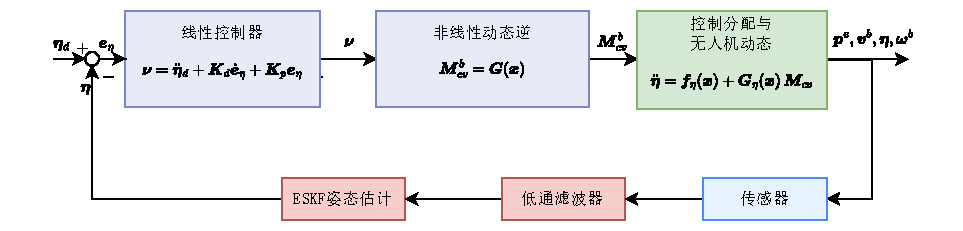
\includegraphics{figure/chapter5/非线性动态逆系统框图.pdf}
    \caption{NDI控制器系统框图}
    \label{fig:NDI_controller}
\end{figure}

通过合理配置 \(\boldsymbol{K}_p\) 和 \(\boldsymbol{K}_d\)，即可使姿态误差按照期望的收敛特性（如临界阻尼或指定带宽）趋近于零。

部署NDI控制器后的系统框图如图\ref{fig:NDI_controller}所示。图中展示了从期望姿态角到控制力矩再到无人机动力学模型的完整信号流向，其中NDI控制律模块依据当前状态估计在线计算非线性逆，实现对姿态通道的解耦与线性化。

在实际实现中，式中的非线性函数 \(\boldsymbol{f}_{\eta}(\boldsymbol{x})\) 和控制效率矩阵 \(\boldsymbol{G}_{\eta}(\boldsymbol{x})\) 需要依据第二章的动力学模型以及第三章辨识得到的气动参数进行计算。由于本文已经通过扩展卡尔曼滤波器在线估计了关键气动参数，NDI控制器能够获得较为准确的先验模型，从而充分发挥其非线性补偿能力。后续仿真将对比NDI控制器与串级PID控制器在典型机动工况下的控制效果，验证其对非线性气动扰动的抑制能力。

% \section{NDI抗扰控制器}
% 本小节针对涵道式无人机在开放环境飞行中的非线性气动力和气动力矩，设计非线性抗扰控制器。
% 阐述开放环境中无人机受到的复杂气动力矩。
% 阐述非线性抗扰控制器的必要性。
% 阐述当前学界普遍使用的INDI控制器\cite{Cheng2024INDI}，相比于INDI控制器，NDI控制器的针对性更强，已有先验模型能够对扰动有较为优异的预判功能。
% 本小节将在仿真环境中验证该抗扰控制器的效果。

% \subsection{NDI控制器介绍}
% 介绍什么是NDI控制器。
% 介绍NDI控制器的原理和结构

\section{INDI控制器与NDI控制器对比实验}

为验证NDI控制器对非线性气动扰动的抑制能力，本小节在第三章所建立的数值仿真环境中开展对比实验。该仿真平台已集成了涵道式无人机的六自由度非线性动力学模型与传感器噪声模型。在此基础上，分别部署了NDI控制器与INDI控制器，其中NDI控制器的设计已在第\ref{sec:NDI_intro}小节中详细阐述，INDI控制器则参考了Cheng等人在涵道式无人机上的相关工作\cite{Cheng2024INDI}。实验过程中，两种控制器保持相同的飞行任务与扰动条件，以公平评估其性能差异。

\subsection{实验设计}

需要指出的是，NDI控制器的实际性能高度依赖于模型精度与状态估计的准确性。为使仿真尽可能贴近真实飞行条件，NDI控制律中的非线性函数 \(\boldsymbol{f}_{\eta}(\boldsymbol{x})\) 与控制效率矩阵 \(\boldsymbol{G}_{\eta}(\boldsymbol{x})\) 并非直接采用仿真模型中的真实状态 \(\boldsymbol{x}\)，而是使用第三章扩展卡尔曼滤波器实时估计出的状态 \(\hat{\boldsymbol{x}}\)。这一设置模拟了实际飞控系统中状态观测器输出存在估计误差的情形，能够更真实地反映NDI控制器在工程应用中的鲁棒性。此外，为模拟飞行过程中的传感器测量噪声，角速度的测量值设定为真实值叠加方差为 \(0.01\,\mathrm{(rad/s)}\) 的高斯白噪声。

\textbf{仿真实验步骤}

1. 初始化：无人机初始状态设置为开放空间中的悬停静止状态，初始姿态角均为零，即\(\phi_0 = \theta_0 = \psi_0 = 0\)，初始角速度为零。

2. 俯仰角阶跃响应：由于俯仰角与滚转角具有对称性，本文仅展示俯仰角的姿态阶跃响应结果。依次轮流给定期望俯仰角 \(\theta_d\) 为 \(20^\circ\) 和 \(0^\circ\) 的阶跃指令，每个指令维持 \(5\,\mathrm{s}\)，重复三次。

3. 偏航角阶跃响应：依次轮流给定期望偏航角 \(\psi_d\) 为 \(30^\circ\) 和 \(0^\circ\) 的阶跃指令，每个指令维持 \(5\,\mathrm{s}\)，重复三次。

 4. 数据采集：仿真过程中以 \(100\,\mathrm{Hz}\) 的频率记录无人机的期望姿态角\(\boldsymbol{\eta}_d\)、实际姿态角\(\boldsymbol{\eta}\)，以及控制力矩\(\boldsymbol{M}_{cv}\)，用于后续分析跟踪曲线。

 \subsection{数据分析}
按照上述实验步骤执行仿真实验后，所得结果经整理，分为横滚角阶跃响应与偏航角阶跃响应两组实验分别展示。对于横滚角阶跃响应，两个控制器的三轴姿态角跟踪曲线对比如图\ref{fig:angle_cmp}所示，对应的控制力矩输出对比如图\ref{fig:effort_cmp}所示。对于偏航角阶跃响应，姿态角跟踪曲线对比如图\ref{fig:angle_cmp_yaw}所示，控制力矩输出对比如图\ref{fig:effort_cmp_yaw}所示。
% 按照上述实验步骤执行仿真实验后，得到的结果经整理，两个控制器的横滚角阶跃响应以及对应的控制量输出对比如图\ref{fig:angle_cmp}和图\ref{fig:effort_cmp}所示，偏航角阶跃响应以及对应的控制量输出对比如图\ref{fig:angle_cmp}和图\ref{fig:effort_cmp}所示。

\begin{figure}[htbp]
    \begin{minipage}{1.0\textwidth}
        \centering
        \includegraphics{matlab/param_recgnize/pdf/NDI_controler_track_roll/cmp_eular_roll.pdf}
        \caption*{(a)横滚角$\varphi$跟随曲线}
    \end{minipage}
    \vspace{0.3cm}
    \begin{minipage}{1.0\textwidth}
        \centering
        \includegraphics{matlab/param_recgnize/pdf/NDI_controler_track_roll/cmp_eular_pitch.pdf}
        \caption*{(b)俯仰角$\theta$跟随曲线}
    \end{minipage}
    \vspace{0.1cm}
    \begin{minipage}{1.0\textwidth}
        \centering
        \includegraphics{matlab/param_recgnize/pdf/NDI_controler_track_roll/cmp_eular_yaw.pdf}
        \caption*{(c)偏航角$\psi$跟随曲线}
    \end{minipage}
    \caption{INDI控制器和NDI控制器横滚角$\varphi$跟随曲线对比}
    \label{fig:angle_cmp}
\end{figure}

\begin{figure}[htbp]
    \begin{minipage}{1.0\textwidth}
        \centering
        \includegraphics{matlab/param_recgnize/pdf/NDI_controler_track_roll/cmp_effort_M_cv_x.pdf}
        \caption*{(a)控制力矩在机体系$X$轴的投影$M_{cv, x}$}
    \end{minipage}
    \vspace{0.3cm}
    \begin{minipage}{1.0\textwidth}
        \centering
        \includegraphics{matlab/param_recgnize/pdf/NDI_controler_track_roll/cmp_effort_M_cv_y.pdf}
        \caption*{(b)控制力矩在机体系$Y$轴的投影$M_{cv, y}$}
    \end{minipage}
    \vspace{0.1cm}
    \begin{minipage}{1.0\textwidth}
        \centering
        \includegraphics{matlab/param_recgnize/pdf/NDI_controler_track_roll/cmp_effort_M_cv_z.pdf}
        \caption*{(c)控制力矩在机体系$Z$轴的投影$M_{cv, z}$}
    \end{minipage}
    \caption{INDI控制器和NDI控制器横滚角$\varphi$跟随实验控制力矩对比}
    \label{fig:effort_cmp}
\end{figure}


\begin{figure}[htbp]
    \begin{minipage}{1.0\textwidth}
        \centering
        \includegraphics{matlab/param_recgnize/pdf/NDI_controler_track_yaw/cmp_eular_roll.pdf}
        \caption*{(a)横滚角$\varphi$跟随曲线}
    \end{minipage}
    \vspace{0.3cm}
    \begin{minipage}{1.0\textwidth}
        \centering
        \includegraphics{matlab/param_recgnize/pdf/NDI_controler_track_yaw/cmp_eular_pitch.pdf}
        \caption*{(b)俯仰角$\theta$跟随曲线}
    \end{minipage}
    \vspace{0.1cm}
    \begin{minipage}{1.0\textwidth}
        \centering
        \includegraphics{matlab/param_recgnize/pdf/NDI_controler_track_yaw/cmp_eular_yaw.pdf}
        \caption*{(c)偏航角$\psi$跟随曲线}
    \end{minipage}
    \caption{INDI控制器和NDI控制器偏航角$\psi$跟随曲线对比}
    \label{fig:angle_cmp_yaw}
\end{figure}

\begin{figure}[htbp]
    \begin{minipage}{1.0\textwidth}
        \centering
        \includegraphics{matlab/param_recgnize/pdf/NDI_controler_track_yaw/cmp_effort_M_cv_x.pdf}
        \caption*{(a)控制力矩在机体系$X$轴的投影$M_{cv, x}$}
    \end{minipage}
    \vspace{0.3cm}
    \begin{minipage}{1.0\textwidth}
        \centering
        \includegraphics{matlab/param_recgnize/pdf/NDI_controler_track_yaw/cmp_effort_M_cv_y.pdf}
        \caption*{(b)控制力矩在机体系$Y$轴的投影$M_{cv, y}$}
    \end{minipage}
    \vspace{0.1cm}
    \begin{minipage}{1.0\textwidth}
        \centering
        \includegraphics{matlab/param_recgnize/pdf/NDI_controler_track_yaw/cmp_effort_M_cv_z.pdf}
        \caption*{(c)控制力矩在机体系$Z$轴的投影$M_{cv, z}$}
    \end{minipage}
    \caption{INDI控制器和NDI控制器偏航角$\psi$跟随实验控制力矩对比}
    \label{fig:effort_cmp_yaw}
\end{figure}

\textbf{横滚角阶跃响应实验分析}

从图\ref{fig:angle_cmp}(a)可以看出，在横滚角阶跃指令下，INDI控制器与NDI控制器的横滚角响应速度基本相当，两者均能在约 \(1.5\,\mathrm{s}\) 内完成对 \(20^\circ\) 阶跃指令的跟踪。

然而，INDI控制器的姿态通道之间存在显著的交叉耦合。观察图\ref{fig:angle_cmp}(b)，当横滚角发生阶跃变化时，INDI控制下的俯仰角出现了约 \(1^\circ\) 的扰动，而NDI控制下的俯仰角则几乎不受影响。这一耦合主要源于涵道风扇高速旋转产生的陀螺力矩效应——横滚角速度的变化会诱发俯仰轴上的干扰力矩，而INDI控制器缺乏对这种耦合机制的前馈补偿，只能被动地依赖姿态环的误差反馈来抑制扰动。相比之下，在已知控制舵面偏转力系数 \(K_{cv}\) 的前提下，NDI控制器通过在线求解逆动力学模型，主动在俯仰通道上输出额外的补偿控制力矩，从而提前抵消了陀螺力矩的耦合影响，如图\ref{fig:effort_cmp}(b)中NDI曲线在横滚阶跃瞬间出现的尖峰所示。

INDI控制器的偏航通道存在明显的初始偏差。从图\ref{fig:angle_cmp}(c)可以看到，在仿真初始阶段，INDI控制下的偏航角出现了高达 \(7^\circ\) 的偏离，随后才逐渐回归期望值。这是由于仿真环境中反扭矩襟翼与涵道风扇的扭矩未能完全相互抵消，而INDI控制器在初始阶段缺少对该力矩残差的前馈补偿，将其视为未知扰动，需要一定时间的在线辨识才能输出有效的抗扰力矩。相比之下，NDI控制器在控制律中直接利用了当前状态估计 \(\hat{\boldsymbol{x}}\) 中的气动参数信息，能够更准确地计算所需的偏航力矩。从图\ref{fig:effort_cmp}(c)可以看出，NDI输出的 \(M_{cv,z}\) 在初始时刻即与INDI输出存在明显差异，这使得偏航角能够迅速稳定在期望值附近，几乎无初始偏移。

此外，INDI控制器的控制输出存在明显的噪声放大问题。从图\ref{fig:effort_cmp}可以看出，INDI控制器输出力矩的噪声幅值明显大于NDI控制器。这是因为INDI控制器需要通过对陀螺仪测量的角速度进行数值差分来获取角加速度，而角速度测量值本身含有噪声，差分操作会进一步放大高频噪声，最终传递至输出力矩。NDI控制器虽然也受到陀螺仪噪声的影响（用于计算陀螺力矩），但由于其不涉及差分过程，噪声未被放大，因此输出力矩的噪声幅值相对较小。在实际飞行中，输出力矩的噪声水平直接影响执行器的能量损耗，且由于舵机存在有限的响应带宽，高频噪声会显著削弱执行器的整体控制效果。

\textbf{偏航角阶跃响应实验分析}

从图\ref{fig:angle_cmp_yaw}(c)可以看出，NDI控制器在偏航通道的响应速度与INDI控制器基本相当，且两者均不存在明显的超调现象。

从图\ref{fig:angle_cmp_yaw}(a)和(b)可以观察到INDI控制器在偏航与俯仰通道之间的耦合现象。在横滚角非零的状态下，当偏航角发生阶跃变化时，根据欧拉角的定义，机体坐标系 \(O_bY_b\) 轴上会产生角速度分量。受陀螺力矩效应影响，该分量将产生作用于俯仰轴的力矩，从而对俯仰角造成扰动。由于INDI控制器缺乏对该扰动力矩的前馈补偿，俯仰角出现了约 \(0.3^\circ\) 以内的波动。相比之下，NDI控制下的俯仰角则保持平稳。此外，图\ref{fig:angle_cmp_yaw}(c)再次验证了INDI控制器在初始阶段的偏航角偏移问题：前 \(2\,\mathrm{s}\) 内存在最大约 \(9^\circ\) 的偏差，并伴有轻微超调。而NDI控制器无此现象，再次体现了在已知反扭矩襟翼系数 \(K_{sta}\) 的情况下NDI控制器的优势。

从图\ref{fig:effort_cmp_yaw}同样可以看出，INDI控制器的控制输出存在明显的噪声放大问题。在实际飞行中，由于舵机存在有限的响应带宽，高频噪声会显著削弱执行器的整体控制效果。

综上所述，仿真结果表明：在模型精确已知且状态估计可信的前提下，NDI控制器能够有效解耦姿态通道之间的非线性耦合，并利用先验模型信息补偿气动参数偏差引起的初始扰动。相较于INDI控制器，NDI控制器在姿态跟踪的稳定性、通道解耦能力以及执行器指令的噪声水平方面均具有显著优势。
% 横滚角阶跃信号响应实验：

% 从图\ref{fig:angle_cmp}横滚角阶跃响应的三轴姿态跟随曲线能够看出，在两个控制器的横滚角响应速度相当的情况下，由于系统呈现出非线性，PID控制器的横滚角和俯仰角、偏航角存在明显的耦合现象，主要体现在，横滚角的姿态变化会给俯仰角带来扰动，俯仰角姿态受到最大$1$度的影响。这主要是陀螺力矩带来的俯仰角和横滚角的耦合。响应地，NDI控制器为了平衡这一作用力，从图\ref{fig:effort_cmp}(b)可以看出，在Y轴会输出额外的控制力矩以平衡该耦合带来的扰动。

% 此外，从图\ref{fig:angle_cmp}(c)可以看出，初始阶段偏航角难以被控制，出现了高达$30$度的偏差。这是由于部署PID控制器时，在初始阶段对反扭矩襟翼的偏转力系数估计不准确，未能准确消除反扭矩襟翼和涵道风扇相抵消后，剩余的Z轴扭矩，经过2s的积分项修正后，偏航角姿态才重新回到期望值附近。响应地，从图\ref{fig:effort_cmp}(c)可以看出，PID控制器和NDI控制器之间的输出存在差距，正是对反扭矩襟翼的偏转力系数估计不准确引起的。

% 偏航角阶跃信号响应实验：

% 从图\ref{fig:angle_cmp_yaw}(c)能够看出，NDI控制器的对每个阶跃信号的响应曲线几乎一致，这反映了其动态特性的一致性。而PID控制器的响应曲线则存在小幅度超调$4$度，且每次偏航角跟随一致性较差。这是由于PID控制器存在积分项，在控制过程中，积分项在实时地动态调整，积分结果取决于上一阶跃响应的误差积分。

% 从图\ref{fig:angle_cmp_yaw}(a)(b)能够看出，仿真实验的初始阶段，横滚角在滚随期望值的过程中，也能看出使用PID控制器时横滚角和俯仰角之间的耦合关系，其表现与横滚角阶跃信号响应实验一致。从图\ref{fig:angle_cmp_yaw}(c)也能看出，使用PID控制器时，初始两秒内，偏航角存在较为明显的误差，这页与横滚角阶跃信号响应实验表现一致。此外，能够从\ref{fig:angle_cmp_yaw}看出，偏航角和其他两个姿态轴的耦合并不明显，PID控制器在跟随偏航角的期望值时，俯仰角的扰动范围在$0.3$度以内。

% \section{本章小结}

% 本章围绕涵道式无人机的抗扰动控制问题，从控制分配、经典PID控制、地面效应补偿到非线性动态逆控制，开展了系统性的设计与验证工作。首先，针对涵道式无人机的过驱动特性，设计了基于伪逆法的控制分配器，实现了期望推力与力矩向执行器指令的合理映射。其次，建立了串级PID控制器作为基础控制框架，并通过试凑法整定参数。针对近地面飞行中的地面效应扰动，基于第四章辨识得到的推力与舵面偏转力随高度变化的模型，提出了动态更新控制效率矩阵的补偿策略。静态台架实验表明，补偿后推力与力矩的稳态误差分别控制在 \(3\%\) 与 \(10\%\) 以内；实飞验证进一步证明，引入补偿后无人机在强地效区的高度与偏航角跟踪性能显著提升，动态品质一致。最后，针对开放环境中的非线性气动耦合问题，设计了非线性动态逆控制器，并在仿真环境中与PID控制器进行了对比。结果表明，NDI控制器能够有效解耦姿态通道间的耦合影响，消除初始气动参数偏差带来的扰动，且具有更好的动态一致性。本章工作为涵道式无人机在全飞行包线内的抗扰控制提供了完整的技术方案与实验支撑。
\section{本章小结}

本章围绕涵道式无人机的抗扰控制问题，从执行器分配、基本姿态位置控制、地面效应补偿到非线性鲁棒控制，构建了完整的控制技术链条。

首先，针对涵道式无人机过驱动的执行器配置，设计了基于伪逆法的控制分配器，将期望推力与期望力矩唯一映射为螺旋桨转速与四个舵面偏转角，为后续控制律的工程实现奠定了基础。其次，设计了串级PID控制器，内环为姿态与角速度环，外环为位置与速度环，通过几何变换实现平动加速度到期望姿态的转换。实际飞行试验表明，该控制器在无地效及弱地效区域内能够保证系统稳定飞行，具有良好的鲁棒性。

针对近地面飞行时地面效应引起的推力增益与舵面效率衰减问题，基于第四章辨识得到的半经验模型，在控制分配环节实时更新推力系数 \(K_{TGE}\) 与舵面偏转力系数 \(K_{cvGE}\)，实现了对地效扰动的动态前馈补偿。静态台架实验表明，补偿后推力与力矩的稳态误差分别控制在 \(3\%\) 与 \(10\%\) 以内；近地面实飞验证进一步证明，引入补偿后无人机在强地效区的高度与偏航角跟踪性能显著提升，稳态误差快速收敛且动态品质一致，有效克服了地效对飞行控制的不利影响。

最后，为应对开放环境中非线性气动耦合与参数不确定性，基于第三章在线辨识得到的关键气动参数，设计了非线性动态逆控制器。仿真对比实验表明，NDI控制器能够主动解耦姿态通道间的陀螺力矩耦合，抑制气动扰动，并利用先验模型信息补偿气动参数偏差带来的初始扰动，在姿态跟踪的通道解耦能力、稳定性和执行器指令的噪声水平方面优于INDI控制器。需要指出的是，受限于样机状态与实验条件，NDI控制器目前仅在仿真环境中完成验证，尚未部署于实际飞行试验，其在实际扰动环境下的控制性能有待进一步检验。

综上，本章所设计的抗扰控制方法兼顾了工程实用性与理论先进性，为涵道式无人机在全飞行包线内的高品质控制提供了系统解决方案。
